 \documentclass[final,3p,times,11pt,onecolumn]{myElsarticle}
\usepackage{float}
\usepackage{times}
\usepackage[utf8]{inputenc}
\usepackage[english]{babel}
\usepackage[T1]{fontenc}
\usepackage{geometry}
\usepackage{color}
\usepackage{soul}
\usepackage{cancel}
\usepackage{subfigure}
\usepackage{enumerate}
\usepackage{amsmath,amsthm,amsfonts,amssymb}
\usepackage{amsthm}
\usepackage{multirow}
\usepackage{graphicx}
\graphicspath{{./figs/}}
\numberwithin{equation}{section}
\usepackage{spverbatim}
\usepackage{fancyhdr}
\usepackage{listings} 
\usepackage{lineno}
\usepackage[none]{hyphenat}
\date{\today}
\setcounter{secnumdepth}{3}
\providecommand{\abs}[1]{\lvert#1\rvert}
\providecommand{\norm}[1]{\lVert#1\rVert}
\setlength\parindent{12pt}		

%\linenumbers

\newcommand{\COM}[1]{{\color{green} #1}}
\newcommand{\HA}[1]{{\color{red} #1}}
\newcommand{\CIP}[1]{{\color{blue} #1}}
\newcommand{\CMV}[1]{{\color{orange} #1}}


\begin{document}

\begin{frontmatter}

\title{A pressure-velocity coupling strategy based on SIMPLEC: the COMPLEX algorithm}
%% A second-neighbour extended correction for segregated p-v coupling algorithms
 
\author[a]{Horacio J. Aguerre}
\author[b,a]{Cesar I. Pairetti}
\author[a,b]{Cesar M. Venier}
\author[a,c]{Santiago Marquez Damian}
\author[a,d]{Norberto M. Nigro}

\address[a]{Centro de Investigación de Métodos Computacionales, CONICET-UNL, Santa Fe, Argentina}
\address[b]{Escuela de Ingenier\'ia Mec\'anica, Facultad de Ciencias Exactas, Ingenieria y Agrimensura, Universidad Nacional de Rosario, Rosario, Argentina}
\address[c]{Facultad Regional Santa Fe, Universidad Tecnologica Nacional, Santa Fe, Argentina}
\address[d]{Facultad de Ingeniería y Ciencias Hídricas, Universidad Nacional del Litoral, Santa Fe, Argentina}

%Start of abstract
\begin{abstract}
This paper introduces a new pressure-velocity coupling algorithm based on the SIMPLEC method. The new approach considers the neighbour velocity corrections of SIMPLEC as a Taylor series expansion, introducing a first-order term to increase the accuracy of the approximation. The new term includes a velocity gradient which is assumed to be a scalar matrix constrained by means of a mass conservation equation.
The stability of the method is analysed via a Fourier decomposition of the error showing a better convergence rate than SIMPLE and SIMPLEC for high relaxation factors. Afterwards, the new method is tested in two typical laminar flow problems where the conclusions of the stability analysis are verified. The current proposal sets a theoretical baseline for further improvements and, in view of the results, it is a promising alternative to improve SIMPLE-like algorithms.
\end{abstract}

\begin{keyword}
Segregated algorithms \sep Segregated method \sep Collocated grids \sep Finite Volume Method 
\end{keyword}
\end{frontmatter}

%%%%%%%%%%%%%%%%%%%%%%%%%%%%%%%%%%%%%
\section{Introduction}

A major numerical difficulty for solving the incompressible Navier-Stokes equations arises from the coupling between
pressure and velocity fields. Several strategies have been proposed to tackle this problem and, in general, they may
be classified into coupled and segregated methods. The first category algorithms consist on solving all the governing
equations at once for all the unknowns in a single system of equations \cite{mazhar1, mazhar2, chen, darwish1, darwish2, uroic}. In these approaches, the pressure and velocity are assembled together in a unique system of equations where the non-linearity of the convective term is treated iteratively. Segregated algorithms, in contrast, solves the equations in a sequential fashion for a unique variable at a time. The procedure is iterative and ends when the unknowns satisfy a certain convergence criterion \cite{ferziger, versteeg, moukalled}. In general, segregated strategies are superior in terms of memory saving and computational performance but their numerical stability may not be guaranteed for solving strongly-coupled physical problems \cite{wang, uroic}. Within these group of methods, the penalty method \cite{temam1968methode}, the artificial compression method \cite{harten1977artificial} and projection methods \cite{chorin1, chorin2, temam1968methode} are among the most adopted in CFD codes nowadays \cite{wang2}. In the projection methods, an initial estimation of the velocity is corrected by means of a pressure equation where the velocity field is forced to satisfy the divergence free condition. The Fractional Step methods (FS) \cite{kim}, for instance, rely on a temporal splitting on the velocity where a first estimate is obtained with the momentum equation using an initial guess of the pressure. Afterwards, the remaining velocity component is computed by solving a pressure equation based on the mass balance.

Under the scope of the projection methods, a new line of strategies was introduced by Patankar and Spalding with the development of the SIMPLE algorithm \cite{patankar1972}. In this method, a pressure equation is derived after introducing the whole momentum equation into the mass balance. Then, the velocity field is updated based on the momentum equation and including the new values of the pressure field. The coupling between pressure and velocity is achieved by means of an iterative procedure where  relaxation factors are needed to improve the stability and convergence rate of the method. Focusing on these last aspects, further improvements have been developed taking the SIMPLE algorithm as a starting
point. Among these, the SIMPLER algorithm \cite{patankar1980} aims to enhance the pressure-velocity coupling by adding an additional pressure equation. Another relevant improvement on SIMPLE was proposed by Van Doormal and Raithby \cite{vanDoormal}, who included an approximation of the neighbour velocity corrections within the pressure equation and velocity update. This algorithm, called SIMPLEC, suppresses the need of relaxing the pressure field after its calculation to guarantee stability. For transient flow problems, Issa proposed the PISO method \cite{issa,issa2} which consists on including corrector sub-steps to enforce mass conservation without relaxing the equations. Many others variants of the SIMPLE method were developed over the years seeking to enhance the robustness and convergence rate of the standard SIMPLE algorithm \cite{tao,qu,cheng2,sun} and their particular advantages and drawbacks can be found in the literature \cite{moukalled, liu, wang}. Despite the aforementioned efforts to improve SIMPLE-like algorithms, the errors introduced by the decoupling of the variables
cannot be completely eliminated which makes the topic still relevant nowadays {\color{red} CITAS RECIENTES (las de la revista, TAO, etc)}.

The error introduced by the SIMPLE algorithm comes from neglecting the neighbour velocity correction in the pressure equation, which is employed to decouple pressure and velocity. If the correction values were known, the discretized system given by the pressure and momentum equations would be equivalent to the original linearized Navier-Stokes problem. In practice, this approximation leads to the need of relaxing the pressure to achieve a stable behaviour towards convergence of the iterative process. Regarding this, the SIMPLEC algorithm avoids relaxing the pressure by considering the neighbour velocity correction equal to the one of the current cell. In other words, it considers the velocity correction as a constant field in the proximities of each cell. The SIMPLEC approximation may be seen as an estimation of the neighbour velocities via a zero-order truncation of a Taylor series expansion. In this context, this work proposes to employ this numerical insight by taking into account a first-order term of the same Taylor series expansion. This approach brings up the need of determining the derivative of the velocity correction, which is a topic of discussion of the present work. This article is organized as follows. Section 2 describes the SIMPLE and SIMPLEC algorithms, which are the starting point for the proposed method. Then, in section 3, the basis and theoretical background of the new method are explained. Subsequently, in section 4, a stability analysis based on Fourier decomposition is performed for the three mentioned algorithms. Next, in Section 5, a series of laminar flow problems are solved to calibrate and investigate the performance of the new proposal. Finally, a discussion of the results and final comments are presented in the last section.

\section{Segregated pressure-velocity coupling methods} \label{sec:theory}

This section presents a general approach for solving the steady state, incompressible Navier-Stokes equations via segregated pressure-based methods. This is done under the framework of the Finite Volume Method (FVM) on collocated grids with the Rhie-Chow correction \cite{rhiechow} and the standard SIMPLE algorithm for the pressure and velocity coupling \cite{patankar1972}. Then, the SIMPLEC algorithm will be introduced \cite{vanDoormal} following the same formalism and focusing on the enhancement of approximating the neighbour velocity corrections for the iterative procedure \cite{moukalled}.

The continuum incompressible Navier-Stokes equations may be written as follows,
\begin{align}
\displaystyle \frac{\partial \boldsymbol{u}}{\partial t} + \nabla \cdotp \boldsymbol{u} \boldsymbol{u} &= -\nabla p + \nu\, \Delta \boldsymbol{u} + \boldsymbol{\Phi},
\label{eq:mom1}
\\
\displaystyle \nabla \cdotp \boldsymbol{u} &= 0, 
\label{eq:mass1}
\end{align}
\noindent where $\displaystyle p = (\mathcal{P}/\rho)$, $\rho$ is the mass density, $\mathcal{P}$ is the pressure field, $\boldsymbol{u}$ is the velocity field, $\nu$ is the kinematic viscosity and $\mathbf{\Phi}$ is a momentum source term.
Based on the FVM, the Eqs.~(\ref{eq:mom1}) and~(\ref{eq:mass1}) may be discretized as:
\begin{align}
a_P\,\boldsymbol{u}_P + \sum_{N} a_{N}\,\boldsymbol{u}_{N} &= b_P\, \boldsymbol{u}^0_P + \boldsymbol{\Phi}_P - \nabla p_P
\qquad \qquad \forall P\,\in\,\Omega,
\label{eq:umom1}
\\
\sum_{f} \boldsymbol{u}_{f} \cdotp \textbf{S}_{f} &= 0
\qquad \qquad \qquad
\qquad \qquad \,\quad \forall P\,\in\,\Omega, 
\label{eq:mass2} 
\end{align}
where the subscript $P$ refers to a given cell of a Finite Volume (FV) mesh $\Omega$, $N$ refers to the values of neighbour cells of $P$ and $f$ refers to values in the faces of the cell $P$, $b_P\, \boldsymbol{u}^0_P$ is the contribution of the previous time-step or iteration and $\textbf{S}_{f}$ is the face-normal vector. Also, $a_P$ and $a_{N}$ are the diagonal and off-diagonal momentum matrix coefficients respectively and the gradient $\nabla p_P$ is computed by linear interpolation of first neighbour values of that field \cite{jasak, moukalled, marquez}. 

Eqs.~(\ref{eq:umom1}) and~(\ref{eq:mass2}) are presented in a way that could serve as a starting point for both steady state and transient algorithm formulations. This is achieved by allowing different definitions of the coefficients $a_P$ and $b_P$ \cite{issa2}. For transient solvers, $b_P$ contains the discretized coefficients of the transient term of the momentum equation (e.g. $b_P = V_P/\Delta t$ for first order schemes) while, for steady state solvers, it is defined following a numerical relaxation of the momentum equations to enhance the stability of the method \cite{moukalled} (e.g. $b_P = \overline{a}_P\,(1-\omega_u)/\omega_u $, where $\overline{a}_P$ have the current cell contributions of the discretization of the advective and diffusive terms of the momentum equation). On the other hand, $a_P = \overline{a}_P + V_P/\Delta t$ for transient solvers and $a_P = \overline{a}_P/\omega_u$ for steady state solvers. Although these dual definitions are still valid for describing steady state (as SIMPLE, SIMPLEC, SIMPLER, etc.) or transient solvers (as PISO), the present work focuses on steady state solvers of the SIMPLE family, so $b_P$ and $a_P$ should be considered as functions of the momentum relaxation factor.

%The value of $b_P$ is function of the temporal scheme in transient solvers and of the relaxation factor in steady-state solvers, ,  
The system given by Eqs.~(\ref{eq:umom1}) and (\ref{eq:mass2}) may be rewritten in a more suitable way for the subsequent numerical approach. First, the current cell velocity $\boldsymbol{u}_{P}$ may be isolated from Eq.~(\ref{eq:umom1}) as,
\begin{equation}
\label{Eq:UpIsolatedH}
\boldsymbol{u}_P
=
\dfrac
{
\boldsymbol{H}_P
- 
\nabla p_P}
{a_P}.
\end{equation}
\noindent where $\boldsymbol{H}_P$ is defined as,
\begin{equation}
\boldsymbol{H}_P
\equiv
-\sum_{N} a_{N}\,\boldsymbol{u}_{N}
+
b_P\, \boldsymbol{u}^0_P 
+ 
\boldsymbol{\Phi}_P
\end{equation}
%Consequently, the Eq.~(\ref{Eq:UpIsolated}) may be expressed as,

Then, Eq.~(\ref{Eq:UpIsolatedH}) is replaced in Eq.~(\ref{eq:mass2}),
\begin{equation}
\sum_{f} 
\left(
\boldsymbol{u}_{P} 
\right)_f
\cdotp 
\textbf{S}_{f} 
=
\sum_{f} 
\left(
\dfrac
{
\boldsymbol{H}_P
- 
\nabla p_P}
{a_P}
\right)_f
\cdotp 
\textbf{S}_{f}
= 
0,
\end{equation}
where the operator $(\cdot)_f$ linearly interpolates the cell values to the faces. Finally, an equation for the pressure field is obtained,
\begin{equation}
\label{Eq:firstPressureEq}
\sum_{f} 
\left(
\dfrac
{
\nabla p_P}
{a_P}
\right)_f
\cdotp 
\textbf{S}_{f}
=
\sum_{f} 
\left(
\dfrac
{
\boldsymbol{H}_P
}
{a_P}
\right)_f
\cdotp 
\textbf{S}_{f}.
\end{equation}
Now, for each cell, there are two system of linearized discrete equations: one for the velocity, given by Eq.~(\ref{Eq:UpIsolatedH}) for each cell, and the other one for the pressure, given by Eq.~(\ref{Eq:firstPressureEq}) for each cell.

Now, for the iterative procedure, a subdivision of the velocity into two contributions is proposed,
\begin{align}
\label{Eq:velocitySubdiv}
\boldsymbol{u}_P
= 
\boldsymbol{u}_P^{*} 
+
\boldsymbol{u}_P^{'} \\
\boldsymbol{u}_N
= 
\boldsymbol{u}_N^{*} 
+
\boldsymbol{u}_N^{'}
\end{align}
where $\boldsymbol{u}^{*}$ is a velocity prediction and $\boldsymbol{u}^{'}$ is a correction of the velocity. This subdivision leads to an analogous separation of the variable $\boldsymbol{H}_P$,
\begin{equation}
\label{Eq:HSubDivision}
\boldsymbol{H}_P 
=
\boldsymbol{H}_P^{*}
+
\boldsymbol{H}_P^{'},
\end{equation}
where,
\begin{align}
\label{Eq:HStar}
\boldsymbol{H}_P^{*} 
&\equiv -\sum_{N} a_{N}\,\boldsymbol{u}_{N}^{*}
+
b_P\, \boldsymbol{u}^0_P 
+ 
\boldsymbol{\Phi}_P,
\\
\label{Eq:HPrima}
\boldsymbol{H}_P^{'}
&\equiv -\sum_{N} a_{N}\,\boldsymbol{u}_{N}^{'}. 
\end{align}
Considering these last expressions, the iterative procedure begins by computing the momentum balance to predict the velocity $\boldsymbol{u}_P^{*}$ using the previous iteration value of the pressure $p^{0}$,
\begin{equation}
\label{Eq:MomentumPredictor}
\boldsymbol{u}_P^{*}
=
\dfrac
{
\boldsymbol{H}_P^*
- 
\nabla p_P^{0}}
{a_P}.
\end{equation}
After this, the pressure is computed by introducing the Eq.~(\ref{Eq:HSubDivision}) in the mass balance of Eq.~(\ref{Eq:firstPressureEq}),
\begin{equation}
\label{Eq:pressureEqSubdiv}
\sum_{f} 
\left(
\dfrac
{
\nabla p_P}
{a_P}
\right)_f
\cdotp 
\textbf{S}_{f}
=
\sum_{f} 
\left(
\dfrac
{
\boldsymbol{H}_P^{*}
+
\boldsymbol{H}_P^{'}
}
{a_P}
\right)_f
\cdotp 
\textbf{S}_{f}.
\end{equation}

\subsection{The SIMPLE algorithm on collocated grids}

Since the correction velocity values $\boldsymbol{u}_N^{'}$  are not yet computed, an approximation of $\boldsymbol{H}_P^{'}$ must be proposed. In this sense, the SIMPLE method proposes to neglect the influence of the neighbour velocity correction which is equivalent to consider,
\begin{equation}
\label{Eq:simpleAproximation}
\boldsymbol{H}_P^{'} = 0,
\end{equation}
thus, introducing~Eq.~(\ref{Eq:simpleAproximation}) into (\ref{Eq:pressureEqSubdiv}),
\begin{equation}
\sum_{f} 
\left(
\dfrac
{
\nabla p_P}
{a_P}
\right)_f
\cdotp 
\textbf{S}_{f}
=
\sum_f 
\left(
\dfrac
{
\boldsymbol{H}_P^*
}
{
a_P
}
\right)_f
\cdot
\boldsymbol{S}_f,
\label{eq:div-free5}  
\end{equation}
which is a Poisson problem for the pressure. Nevertheless, for collocated grids, solving this system in a straightforward manner may lead to high-frequency oscillations. The Rhie-Chow correction \cite{rhiechow} seeks to reduce this effect by introducing a stabilizing term, 

\begin{equation}
\label{eq:pEqnSIMPLE2}
\sum_{f} 
\left(
\dfrac
{
\nabla p_P}
{a_P}
\right)_f
\cdotp 
\textbf{S}_{f} 
=
\sum_f 
\left(
\dfrac{
\boldsymbol{H}_P^*
}
{
a_P
}
\right)_f
\cdot
\boldsymbol{S}_f 
+
\sum_f  
\left[
\left(
\frac{\nabla p_P}{a_P}
\right)_f
- 
\left(
\frac{1}{a_P}
\right)_f 
\nabla p_f
\right]
\cdot 
\boldsymbol{S}_f.
\end{equation}
Reordering the terms in Eq.~(\ref{eq:pEqnSIMPLE2}) leads to the following form for the pressure equation,
\begin{equation}\label{eq:pEqnSIMPLE3}
\sum_f \left(\frac{1}{a_P}\right)_f \nabla p_f 
\cdot
\boldsymbol{S}_f 
=  \sum_f \left(\frac{\boldsymbol{H}_P^*}{a_P}\right)_f \cdot \boldsymbol{S}_f.
\end{equation}
For SIMPLE, the pressure field is usually relaxed after its calculation in Eq.~(\ref{eq:pEqnSIMPLE3}) to improve the numerical stability of the method, following,
\begin{equation}
\label{eq:relaxP}
p_P
=
\omega_P p_P^{BR} + (1-\omega_P) p_P^0.
\end{equation}
\noindent where $p_P^{BR}$ is the pressure field obtained from Eq.~(\ref{eq:pEqnSIMPLE3}) (before relaxation).

Finally, the velocity value is computed through Eq.~(\ref{Eq:UpIsolatedH}) where the variable $\boldsymbol{H}_P$ is approximated by $\boldsymbol{H}_P^{*}$ (as was done in the mass balance equation),
\begin{equation}
\label{eq:SIMPLECorr}
\boldsymbol{u}_P
=
\dfrac
{
\boldsymbol{H}_P^*
- 
\nabla p_P}
{a_P}.
\end{equation}
Note that last equation is explicit since the terms r.h.s of last equation are known. The algorithm continues iteratively from Eq.~(\ref{Eq:MomentumPredictor}), where $\boldsymbol{u}_P^0$ and $p_P^0$ are replaced by the values of $\boldsymbol{u}_P$ and $p_P$ from the previous iteration, until a certain convergence criteria is reached.

% In order to do so, the velocity field $\boldsymbol{u}_P$, originally on cell-centers, needs to be interpolated to the faces obtaining: 
%
% \begin{equation}
% \begin{split}
% \sum_{f} \left( \boldsymbol{H}_P_P - \frac{1}{a_P} \nabla p_P  \right)_f \cdotp \textbf{S}_{f} = 0 
% \end{split}
% \label{eq:pEq1} 
% \end{equation}
%
%Therefore, the Corrector step may be summarized as:
%
%\begin{enumerate}
%
%\item Assemble and solve the pressure based on Eq.~(\ref{eq:pEq1}):
%
%\begin{equation}
%\begin{split}
%\sum_{f} \left( \frac{1}{a_P} \nabla p'_P \right)_f \cdotp \textbf{S}_{f} = \sum_{f} \boldsymbol{u}^*_f \cdotp \textbf{S}_{f}
%\end{split}
%\label{eq:pEq2} 
%\end{equation}


%\CIP{Si conservamos la forma relativa, aquí habría que meter la explicación de Rhie Chow}

%\item {\color{red}Compute} the face fluxes by adding the new pressure contribution:
%
%\begin{equation}
%\begin{split}
%F_f = \boldsymbol{u}^*_f \cdotp \textbf{S}_{f} -  \left( \frac{1}{a_P}\right)_f \nabla p'_f  \cdotp \textbf{S}_{f}
%\end{split}
%\label{eq:Fhat} 
%\end{equation}
%
%\item Correct the cell-centered velocity field based on the new pressure field, using Eq. (\ref{eq:umom3b})
%
%\begin{equation}\label{eq:umom3b}
%\begin{split}
%\boldsymbol{u}_P = \boldsymbol{u}^*_P - \frac{1}{a_P} \nabla p'_P 
%\end{split}
%\end{equation}
%
%\end{enumerate}

%\fi
%Most of the SIMPLE-family algorithms preserve this general structure. In particular, the SIMPLE algorithm \cite{patankar1972}, originally conceived as a steady state flow solver, adds under-relaxation factors to obtain a stable solution. Another variant is the PISO {\color{red}(Pressure-Implicit with Splitting of Operators)} algorithm, which relies on iterating the Corrector step a given number of times to ensure a correct coupling between pressure and velocity for transient flow problems \cite{issa,issa2}. {\color{red} The SIMPLE-PISO combined technique has been largely adopted in several computational codes (e.g. OpenFOAM(R) \cite{ofpg}) to address transient incompressible flow problems due to its beneficial convergence features. It consists on iterating the corrector steps until a certain mass conservation criteria is fulfilled (as in PISO) and iterating the whole sequence (Momentum Predictor and Corrector Step) several times until both mass and momentum equations are verified for each time step. This algorithm will be adopted in the present work.}

\subsection{Improving the neighbour approximation: the SIMPLEC algorithm}
The SIMPLEC~\cite{vanDoormal} algorithm proposes an approximation for the neighbour velocity correction $\boldsymbol{u}_N'$,
\begin{equation}
\label{Eq:simplecAproximation}
\boldsymbol{u}_N'
=
\boldsymbol{u}_P'
\end{equation}
and therefore the Eq.~(\ref{Eq:HPrima}) may be expressed as,
\begin{equation}
\label{eq:H_SIMPLEC}
\boldsymbol{H}_P'= \left(-\sum_N a_N\right) \boldsymbol{u}'_P.
\end{equation}
To include it in Eq.~(\ref{Eq:pressureEqSubdiv}), first it must be written in terms of the pressure gradient. To do this, an expression for $\boldsymbol{u}_P^{'}$ is derived by subtracting Eq.~(\ref{Eq:MomentumPredictor}) from Eq.~(\ref{Eq:UpIsolatedH}),
\begin{equation}
\label{Eq:UPrimaIsolated}
\boldsymbol{u}_P'
=
\dfrac
{
\boldsymbol{H}_P'
- 
\left(
\nabla p_P
-
\nabla p_P^{0}
\right)
}
{a_P},
\end{equation}
which, in combination with Eq.~(\ref{eq:H_SIMPLEC}), provides an expression for $\boldsymbol{H}_P'$ as function of the pressure gradient,
\begin{equation}
\label{Eq:HPrima2}
\boldsymbol{H}_P'
= 
\dfrac
{
\left(
\tilde{a}_P
-
a_P
\right)
}
{
\tilde{a}_P
}
\left(
\nabla p_P
-
\nabla p_P^{0}
\right).
\end{equation}
where,
\begin{equation}
\tilde{a}_P
=
a_P + \sum_{N} a_{N}.
\end{equation}
Subsequently, introducing Eq.~(\ref{Eq:HPrima}) in Eq.~(\ref{Eq:pressureEqSubdiv}),

\begin{equation}
\label{Eq:pressureReplacedSimplec}
\sum_{f} 
\left(
\dfrac
{
\nabla p_P}
{a_P}
\right)_f
\cdotp 
\boldsymbol{S}_{f}
=
\sum_{f} 
\left(
\dfrac
{
\boldsymbol{H}_P^{*}
}
{a_P}
\right)_f
\cdotp 
\boldsymbol{S}_{f}
+
\sum_f
\left[
\dfrac
{
\left(
\tilde{a}_P
-
a_P
\right)
}
{
\tilde{a}_P\,a_P
}
\left(
\nabla p_P
-
\nabla p_P^{0}
\right)
\right]_f
\cdot
\boldsymbol{S}_{f},
\end{equation}
which may be rewritten as,
\begin{equation}
\label{Eq:pressureReplacedSimplec2}
\sum_{f} 
\left(
\dfrac
{
\nabla p_P}
{\tilde{a}_P}
\right)_f
\cdotp 
\boldsymbol{S}_{f}
=
\sum_{f} 
\left(
\dfrac
{
\boldsymbol{H}_P^{*}
}
{a_P}
\right)_f
\cdotp 
\boldsymbol{S}_{f}
+
\sum_f
\left[
\left(
\dfrac{1}
{\tilde{a}_P}
-
\dfrac{1}
{a_P}
\right)
\nabla p^{0}
\right]_f
\cdot
\boldsymbol{S}_f.
\end{equation}
The pressure equation is obtained by including an analogous Rhie-Chow correction:

\begin{equation}
\label{eq:pEqnSIMPLEC2}
\begin{array}{ccc}
&
\sum_{f} 
\left(
\dfrac
{
\nabla p_P}
{\tilde{a}_P}
\right)_f
\cdotp 
\boldsymbol{S}_{f} 
=
\sum_{f} 
\left(
\dfrac
{
\boldsymbol{H}_P^{*}
}
{a_P}
\right)_f
\cdotp 
\boldsymbol{S}_{f}
+
\sum_f
\left[
\left(
\dfrac{1}
{\tilde{a}_P}
-
\dfrac{1}
{a_P}
\right)
\nabla p^{0}
\right]_f
\cdot
\boldsymbol{S}_f
&
\\
&+& \\
&
\sum_f
\left\lbrace
\left(
\dfrac
{
\nabla p
}
{\tilde{a}_P}
\right)_f
-
\left(
\dfrac
{1}
{\tilde{a}_P}
\right)_f
\nabla p_f
+
\left(
\dfrac
{1}
{\tilde{a}_P}
-
\dfrac
{1}
{a_P}
\right)_f
\nabla p^{0}_f
-
\left[
\left(
\dfrac
{1}
{\tilde{a}_P}
-
\dfrac
{1}
{a_P}
\right)
\nabla p^0
\right]_f
\right\rbrace
\cdot
\boldsymbol{S}_f,
&
\end{array}
\end{equation}
which may be simplified as,
\begin{equation}
\sum_f
\left(
\dfrac
{1}
{\tilde{a}_P}
\right)_f
\nabla p_f
\cdot 
\boldsymbol{S}_f
= 
\sum_f 
\left(
\frac{
\boldsymbol{H}_P^*
}{a_P}
\right)_f 
\cdot
\boldsymbol{S}_f
+
\sum_f
\left[
\left(
\dfrac
{1}
{\tilde{a}_P}
-
\dfrac
{1}
{a_P}
\right)_f
\nabla p^{0}_f
\right]
\cdot
\boldsymbol{S}_f.
\label{eq:pEqnSIMPLEC}
\end{equation}

The velocity is computed by including the approximation of Eq.~(\ref{Eq:HPrima2}) into Eq.~(\ref{Eq:UpIsolatedH}):

\begin{equation}
\label{eq:uCorrSIMPLEC}
\boldsymbol{u}_P 
=
\dfrac
{
\boldsymbol{H}_P^*
- 
\nabla p_P}
{a_P}
+
\dfrac
{
\left(
\tilde{a}_P
-
a_P
\right)
}
{
\tilde{a}_P\,a_P
}
\left(
\nabla p_P
-
\nabla p_P^{0}
\right).
\end{equation}
where the terms may be reordered to obtain,
\begin{equation}
\label{Eq:velocitySimplec}
\boldsymbol{u}_P 
=
\dfrac
{
\boldsymbol{H}_P^*
- 
\nabla p_P}
{\tilde{a}_P}
+
\left(
\dfrac{1}
{\tilde{a}_P}
-
\dfrac{1}
{a_P}
\right)
\nabla p^{0}.
\end{equation}


The reader may notice that the only difference between SIMPLE and SIMPLEC is in the presence of a coefficient $\tilde{a}_P$ different from $a_P$. This modification represents a significant improvement in the stability and convergence properties of the algorithm, which matches with the performance of the SIMPLE method with optimal setting of the relaxation factors \cite{miller1}. In fact, SIMPLEC do not uses pressure relaxation factors since they are not needed to ensure stability (as for SIMPLE). 

In the same spirit, this work proposes a new pressure-velocity coupling method of the SIMPLE family, based on increasing the order of approximation of the neighbour velocity corrections.

\section{A COupling Method for Pressure Linked Equations based on series eXpansions: COMPLEX}
\label{sec:COMPLEX}

In order to accurately estimate the contribution of the neighbour velocity corrections, an approximation is proposed based on preserving first order terms of a Taylor series expansion over $\boldsymbol{u}_N'$,
\begin{equation}\label{eq:uNTaylor}
\boldsymbol{u}_N' = \boldsymbol{u}_P' + \boldsymbol{x}_{PN}\cdot 
\nabla \boldsymbol{u}_f'.
\end{equation}
where $\boldsymbol{x}_{PN}$ is a distance vector that goes from the cell centroid $P$ to the cell centroid $N$.

Thus, the $\boldsymbol{H}_P'$ variable may be written as,
\begin{equation}
\label{Eq:HPrimaComplex}
\boldsymbol{H}_P'
=
\left(
-\sum_N a_N
\right)
\boldsymbol{u}_P' 
+
\left(
-\sum_N a_N
\right)
\left(
\boldsymbol{x}_{PN}\cdot 
\nabla \boldsymbol{u}_f'
\right),
\end{equation}
which combined with Eq.~(\ref{Eq:UPrimaIsolated}) leads to,
\begin{equation}
\label{Eq:HPrimaComplexReady}
\boldsymbol{H}_P'
= 
\dfrac
{
\left(
\tilde{a}_P
-
a_P
\right)
}
{
\tilde{a}_P
}
\left(
\nabla p_P
-
\nabla p_P^{0}
\right)
+
\dfrac{a_P}{\tilde{a}_P}
\,
\boldsymbol{\delta}_P,
\end{equation}
where $\boldsymbol{\delta}_P$ is defined as the second term of the r.h.s of Eq.~(\ref{Eq:HPrimaComplex}), which will be referred to as Complex term,
\begin{equation}
\boldsymbol{\delta}_P 
\equiv 
\left(
-\sum_N a_N
\right)
\left(
\boldsymbol{x}_{PN}\cdot 
\nabla \boldsymbol{u}_f'
\right),
\end{equation}
Including Eq.~(\ref{Eq:HPrimaComplexReady}) in Eq.~(\ref{Eq:pressureEqSubdiv}) and following an analogous derivation as done from Eq.~(\ref{Eq:pressureReplacedSimplec}) up to Eq.~(\ref{eq:pEqnSIMPLEC}), the following pressure equation is obtained,
\begin{equation}
\label{Eq:pressureComplex}
\sum_f
\left[
\left(
\dfrac
{1}
{\tilde{a}_P}
\right)_f
\nabla p_f
\right]
\cdot 
\boldsymbol{S}_f
= 
\sum_f 
\left[
\frac{1}{a_P}
\left(
\boldsymbol{H}_P^*
\right)
\right]_f 
\cdot
\boldsymbol{S}_f
+
\sum_f
\left[
\left(
\dfrac
{1}
{\tilde{a}_P}
-
\dfrac
{1}
{a_P}
\right)_f
\nabla p^{0}_f
\right]
\cdot
\boldsymbol{S}_f
+
\sum_f
\left(
\dfrac{\boldsymbol{\delta}_P}{\tilde{a}_P}
\right)_f
\cdot
\boldsymbol{S}_f.
\end{equation}
Then, the velocity is computed including the approximation of Eq.~(\ref{Eq:HPrimaComplex}) in Eq.~(\ref{Eq:UpIsolatedH}),
\begin{equation}
\label{Eq:velocityComplex}
\boldsymbol{u}_P 
=
\dfrac
{
\boldsymbol{H}_P^*
- 
\nabla p_P}
{\tilde{a}_P}
+
\left(
\dfrac{1}
{\tilde{a}_P}
-
\dfrac{1}
{a_P}
\right)
\nabla p^{0}
+
\dfrac{\boldsymbol{\delta}_P}
{\tilde{a}_P}.
\end{equation}
The Eqs.~(\ref{Eq:pressureComplex}) and (\ref{Eq:velocityComplex}) are similar to Eqs.~(\ref{eq:pEqnSIMPLEC}) and (\ref{Eq:velocitySimplec}) respectively but for the Complex term $\boldsymbol{\delta}_P$ which has as main unknown the face gradient $\nabla \boldsymbol{u}_f'$. Putting aside the task of computing this term, this means that the general structure of the SIMPLEC algorithm remains unaltered. 

\subsection{Computation of the face gradient}
The face gradient $\nabla \boldsymbol{u}_f' $ is obtained as a linear interpolation of a cell-centred gradient $\nabla \boldsymbol{u}_P'$,
\begin{equation}
\label{Eq:UFaceGradient}
\nabla \boldsymbol{u}_f'
=
(\nabla \boldsymbol{u}_P')_f.
\end{equation}
To obtain an expression for the cell-centred gradient, a derivation starts by including the subdivision of the velocity given in Eq.~(\ref{Eq:velocitySubdiv}) in the mass balance given of Eq.~(\ref{eq:mass2}),
\begin{equation}
\label{Eq:massEqSubdivided}
\sum_{f} 
\left(
\boldsymbol{u}_{P}^*
+ 
\boldsymbol{u}_{P}'
\right)_f
\cdotp \textbf{S}_{f} 
=
\sum_{f} 
\left(
\boldsymbol{u}_{P}^*
\right)_f
\cdotp \textbf{S}_{f}
+
\sum_{f} 
\left(
\boldsymbol{u}_{P}'
\right)_f
\cdotp \textbf{S}_{f}
=
0
\end{equation}
In this last equation, the face values $\left(\boldsymbol{u}_P'\right)_f$ can expressed as function of $\nabla \boldsymbol{u}_P'$ by considering the following first-order Taylor expansion,
\begin{equation}
\label{Eq:TaylorOnFace}
\left(
\boldsymbol{u}_P'
\right)_f
=
\boldsymbol{u}_P'
+
\boldsymbol{x}_{Pf}
\cdot 
\nabla \boldsymbol{u}_P'.
\end{equation} 
Now, this may be introduced in Eq.~(\ref{Eq:massEqSubdivided}),
\begin{align}
\sum_f 
\left(
\boldsymbol{u}_P'
+
\boldsymbol{x}_{Pf}
\cdot 
\nabla \boldsymbol{u}_P'
\right)
\cdot 
\boldsymbol{S}_f 
&=
-\sum_f
\left(
\boldsymbol{u}_P^{*}
\right)_{f} 
\cdot 
\boldsymbol{S}_f
\\
\boldsymbol{u}_P'
\cdot 
\sum_f 
\boldsymbol{S}_f
+
\sum_f 
\left(
\boldsymbol{x}_{Pf}
\cdot 
\nabla \boldsymbol{u}_P'
\right)
\cdot 
\boldsymbol{S}_f
&=
-\sum_f
\left(
\boldsymbol{u}_P^{*}
\right)_{f} 
\cdot 
\boldsymbol{S}_f
\\
\label{Eq:Last}
\sum_f 
\left(
\boldsymbol{x}_{Pf}
\cdot 
\nabla \boldsymbol{u}_P'
\right)
\cdot 
\boldsymbol{S}_f
&=
-\sum_f
\left(
\boldsymbol{u}_P^{*}
\right)_{f} 
\cdot 
\boldsymbol{S}_f
\end{align}
where $\sum_f \boldsymbol{S}_f = \boldsymbol{0}$ for closed polyhedrons and $\boldsymbol{u}_P^{*}$ is known from Eq.~(\ref{Eq:MomentumPredictor}),
\begin{equation}
\left(
\boldsymbol{u}_P^{*}
\right)_{f}
=
\left[\frac{1}{a_P}\left(\boldsymbol{H}_P^* - \nabla p_P^{0}\right)\right]_f.
\end{equation}
Now, a similar form of the Rhie-Chow correction term, given in Eq.~(\ref{eq:pEqnSIMPLE2}), is included,
\begin{equation}
\left(
\boldsymbol{u_P}^{*}
\right)_{f}
=
\left[\frac{1}{a_P}\left(\boldsymbol{H}_P^* - \nabla p_P^{0}\right)\right]_f
+
\left[
\left(
\frac{\nabla p_P^{0}}{a_P}
\right)_f
- 
\left(
\frac{1}{a_P}
\right)_f 
\nabla p_f^{0} 
\right],
\end{equation}
leading to, 
\begin{equation}
\left(
\boldsymbol{u_P}^{*}
\right)_{f}
=
 \left(\frac{\boldsymbol{H}_P^*}{a_P}\right)_f 
 -
 \left(\frac{1}{a_P}\right)_f \nabla p_f^{0}.
\end{equation}
Then, replacing this expression into Eq.~(\ref{Eq:Last}),
\begin{equation}
\label{Eq:mainGradEq}
\sum_f 
\left(
\boldsymbol{x}_{Pf}
\cdot 
\nabla \boldsymbol{u}_P'
\right)
\cdot 
\boldsymbol{S}_f
=
-\sum_f
\left[
\left(\frac{\boldsymbol{H}_P^*}{a_P}\right)_f 
 -
 \left(\frac{1}{a_P}\right)_f \nabla p_f^{0}
 \right]
\cdot 
\boldsymbol{S}_f.
\end{equation}
This last equation allows to compute the cell gradient $\nabla \boldsymbol{u}_P'$ as a function of $\boldsymbol{H}_P^*$ and $\nabla p_f^{0}$ which are known values after the first step of the algorithm. However, the Eq.~(\ref{Eq:mainGradEq}) is underdetermined since the gradient $\nabla \boldsymbol{u}_P'$ is a second order tensor with nine unknown scalar values. In order to solve this, an additional approximation is proposed: 
\begin{equation}
\nabla \boldsymbol{u}_P'
=
\alpha_P\,
\boldsymbol{I}
\label{eq:gradApprox}
\end{equation}
This means that the gradient of the velocity corrections is considered to be a diagonal isotropic matrix. Therefore, it has only one unknown scalar value.
Replacing this last definition in Eq.~(\ref{Eq:mainGradEq}) leads to,
\begin{align}
\sum_f 
\left(
\boldsymbol{x}_{Pf}
\cdot 
\alpha_P\,
\boldsymbol{I}
\right)
\cdot 
\boldsymbol{S}_f
&=
-\sum_f
\left[
\left(\frac{\boldsymbol{H}_P^*}{a_P}\right)_f 
 -
 \left(\frac{1}{a_P}\right)_f \nabla p_f^{*}
 \right]
\cdot 
\boldsymbol{S}_f,
\\
\alpha_P
\sum_f 
\left(
\boldsymbol{x}_{Pf}
\cdot 
\boldsymbol{I}
\right)
\cdot 
\boldsymbol{S}_f
&=
-\sum_f
\left[
\left(\frac{\boldsymbol{H}_P^*}{a_P}\right)_f 
 -
 \left(\frac{1}{a_P}\right)_f \nabla p_f^{*}
 \right]
\cdot 
\boldsymbol{S}_f,
\end{align}
and isolating $\alpha_P$,
\begin{equation}
\alpha_P
=
\dfrac
{-\sum_f
\left[
\left(\frac{\boldsymbol{H}_P^*}{a_P}\right)_f 
 -
 \left(\frac{1}{a_P}\right)_f \nabla p_f^{*}
 \right]
\cdot 
\boldsymbol{S}_f}
{\sum_f 
\boldsymbol{x}_{Pf}
\cdot 
\boldsymbol{S}_f}
\end{equation}

Finally, the face gradient given by Eq.~(\ref{Eq:UFaceGradient}) may be computed using the face interpolated values of $\alpha$,
\begin{equation}
\label{Eq:scalarMatrix}
\nabla \boldsymbol{u}_f'
=
\left(
\alpha_P
\right)_f
\boldsymbol{I}.
\end{equation}

\subsection{Relaxation of the Complex term}
The COMPLEX method is based on an approximation of the neighbours velocity corrections $\boldsymbol{u}_N'$ based on a Taylor expansion and taking into account the mass balance equation. However, an accurate definition of the gradient for the second term of the Taylor expansion requires additional information which is not available before solving the pressure equation. The only accurate information that can be extracted from this approach is the trace of the gradient of the velocity correction, which is opposite to the divergence of the predicted velocity $\boldsymbol{u}^*$. Due to this numerical difficulty, the approximation given in Eq.~(\ref{eq:gradApprox}) provides the mathematical closure of the numerical problem at the cost of reducing the potential of the original proposal. The physical meaning of using a scalar matrix as an estimate of the gradient of the velocity is that the deformation of the velocity correction is considered to be isotropic. This may not be true once the velocity field is computed with the new pressure values. Taking this into account, a relaxation of the complex term $\boldsymbol{\delta}_P$ is proposed in order to avoid an overestimation of the real value of $\boldsymbol{u}_N'$. Introducing a relaxation factor on the Complex term in the Eqs.~(\ref{Eq:pressureComplex}) and (\ref{Eq:velocityComplex}) , 
\begin{equation}
\label{Eq:pressureComplexRelaxed}
\sum_f
\left[
\left(
\dfrac
{1}
{\tilde{a}_P}
\right)_f
\nabla p_f
\right]
\cdot 
\boldsymbol{S}_f
= 
\sum_f 
\left[
\frac{1}{a_P}
\left(
\boldsymbol{H}_P^*
\right)
\right]_f 
\cdot
\boldsymbol{S}_f
+
\sum_f
\left[
\left(
\dfrac
{1}
{\tilde{a}_P}
-
\dfrac
{1}
{a_P}
\right)_f
\nabla p^{0}_f
\right]
\cdot
\boldsymbol{S}_f
+
\kappa
\sum_f
\left(
\dfrac{\boldsymbol{\delta}_P}{\tilde{a}_P}
\right)_f
\cdot
\boldsymbol{S}_f.
\end{equation}
\begin{equation}
\label{Eq:velocityComplexRelaxed}
\boldsymbol{u}_P 
=
\dfrac
{
\boldsymbol{H}_P^*
- 
\nabla p_P}
{\tilde{a}_P}
+
\left(
\dfrac{1}
{\tilde{a}_P}
-
\dfrac{1}
{a_P}
\right)
\nabla p^{0}
+
\kappa
\dfrac{\boldsymbol{\delta}_P}
{\tilde{a}_P}.
\end{equation}
where $\kappa$ is the Complex relaxation factor and its value is between 0 and 1.

\section{Stability Analysis}
\label{sec:fourier}

In order to investigate the features of the new method, a stability analysis based on a Fourier decomposition of the error is proposed. This technique has proven to be a powerful tool to determine the numerical and physical conditions that guarantee a stable solution for linearized equations. Moreover, the methodology is extendable for the analysis of multi-variable discrete systems that are addressed by segregation of the variables. The main feature of this approach is to condense the spatial information into a frequency spectrum where only the term of the frequency that produces the highest amplification of the error is taken into account. In this way, the problem is reduced to the analysis of the Fourier coefficients and its evolution in time \cite{hirsch}. 

On the downside, this technique relies on having constant coefficients in the momentum and pressure equations, which will be constant up to the point of the beginning of the second iteration where $a_P$ and $a_N$ are updated with the new velocity field. That means that a sequence of several SIMPLE iterations cannot be studied via a Fourier decomposition as a whole. Instead, each iteration need to be studied separately. Another drawback of the Fourier analysis is that only periodic boundary conditions can be considered for the analysis. Nevertheless, these restrictions are the price to pay to have an analytical tool that gives valuable information about the ranges of stability and error damping of each method as a function of just a few parameters. Moreover, since this technique will be used to compare each coupling method under the same conditions, these drawbacks will become irrelevant.

Many examples of the usage of this technique can be found in the literature. Shaw et al. \cite{shaw} used it to study the error damping properties of the SIMPLE algorithm in staggered grids. Then, Miller \cite{miller1} extended this analysis to the investigation of the performance of SIMPLE and SIMPLEC on both, collocated and staggered grids. On the other hand, Liu et al. \cite{liu} adopted the same technique to study a large number of algorithms of the SIMPLE family. More recently, Miller et al. \cite{miller2} extended this technique to study Eulerian multiphase flow models, while Venier et al. \cite{venier} studied the stability features of the PISO algorithm for addressing transient and steady state flow problems.

Here, a single iteration of the algorithm will be studied, which can be separated into three stages: the momentum predictor, the pressure equation and the velocity update. The equations of each stage (for each method) will be written in its Fourier decomposed form (with only the term with the frequency that produces the highest amplification). In order to do so, first, these equations are written in terms of the errors of the variables (i.e. pressure and velocity), which are defined as:
\begin{equation}
    e^k_{\phi,M} = \phi^{exact}_{M}-\phi_M^{k},
\end{equation}
where $k$ is a given stage of the sequence ($0$ for the initial values, * for the variables after the momentum predictor, ** for the variables after the pressure equation and *** for the variables after the velocity update), $\phi$ is a given variable (pressure or velocity) and $M$ represents the spatial location.
The present study will be done for a one-dimensional FV discretization (see Fig. \ref{fig:4a}) to simplify the analysis.% and arrive to some preliminary conclusions about the stability features of the method. Later on, all the methods will be tested in benchmark problems and the stability and convergence rate will be fully assessed.
\begin{figure}[t!]
    \centering
    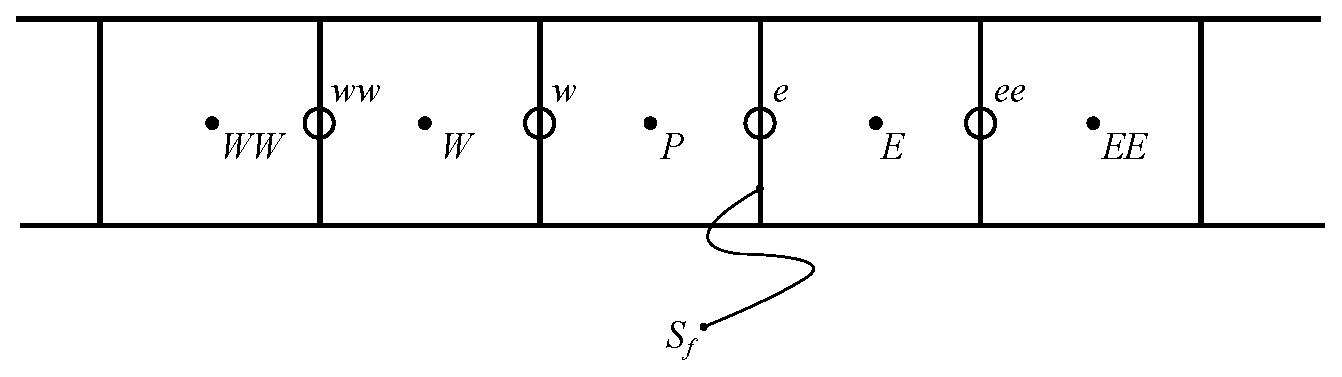
\includegraphics[width=0.7\textwidth]{fig/cells.eps}
    \caption{One-dimensional FVM discretization.}
    \label{fig:4a}
\end{figure}

First, the momentum predictor (Eq. (\ref{Eq:MomentumPredictor})) will be rewritten in terms of the error of the variables as follows,
\begin{equation}
    \dfrac{\overline{a}_P}{\omega} \; u_P^* + a_E \; u_E^* + a_W \; u_W^* = \dfrac{1-\omega}{\omega} \; \overline{a}_P \; u_P^0 - (\hat{\nabla} p)_P + \Phi_P,
\end{equation}
\begin{equation}
    \dfrac{\overline{a}_P}{\omega} \; e_{u,P}^* + a_E \; e_{u,E}^* + a_W \; e_{u,W}^* = \dfrac{1-\omega}{\omega} \; \overline{a}_P \; e_{u,P}^0 - \dfrac{S_f}{2} (e^0_{p,E}-e^0_{p,W}),
    \label{eq:MPerror}
\end{equation}
where $P$, $W$ and $E$ represents the main cell and neighbour cells respectively on this current FVM stencil (see Fig. \ref{fig:4a}).
Now, the errors may be written in terms of the Fourier decomposition as:
\begin{equation}
    e^k_{\phi,M} = \alpha^k_{\phi} \; \text{e}^{\left( i \, \theta \, \frac{x_M}{\Delta x}\right)},
    \label{eq:error}
\end{equation}
which, for multivariable systems, becomes:
\begin{equation}
\begin{bmatrix}
e_u \\
e_p 
\end{bmatrix}^{k}
=
\begin{bmatrix}
u \\
p 
\end{bmatrix}^{n+1}
-\begin{bmatrix}
u \\
p 
\end{bmatrix}^{k}
=
\begin{bmatrix}
\alpha_u \\
\alpha_p 
\end{bmatrix}^{k}
\; \text{e}^{\left( i \, \theta \, \frac{x_M}{\Delta x}\right)},
\label{eq:fou1}
\end{equation}
where $\Delta x$ represents the distance between the centroids of two adjoining cells.
Replacing each error on Eq.~(\ref{eq:MPerror}) for its corresponding Fourier decomposition, as given by Eq. (\ref{eq:error}), the following equation is obtained:
\begin{equation}
    P_u \alpha_u^* = \left( \dfrac{1-\omega}{\omega} \; \overline{a}_P \right) \; \alpha_u^0 + \left(- \dfrac{S_f}{2} \right) \left(\text{e}^{i \theta} -  \text{e}^{-i \theta} \right) \alpha_p^0,
    \label{eq:MPfou}
\end{equation}
where,
\begin{equation}
P_u = \dfrac{\overline{a}_P}{\omega}  + a_E \; \text{e}^{i \theta} + a_W \; \text{e}^{-i \theta}.
\end{equation}

This may be rewritten as,
\begin{equation}
     \alpha_u^* = a_1 \alpha_u^0 + b_1 \alpha_p^0,
    \label{eq:MPfou2}
\end{equation}
where:
\begin{equation}
\begin{split}
     a_1 &= \dfrac{1-\omega}{\omega} \; \overline{a}_P \; P_u^{-1},
\\
b_1 &= - \left( \dfrac{S_f}{2} \right) \left( \text{e}^{i \theta} -  \text{e}^{-i \theta} \right) \; P_u^{-1},
\end{split}
\end{equation}
and since $p^* = p^0$, the following amplification system is obtained:
\begin{equation}
\begin{bmatrix}
\alpha_u \\
\alpha_p 
\end{bmatrix}^{*} =
\begin{bmatrix}
a_1 & b_1 \\
0 & 1
\end{bmatrix}
\begin{bmatrix}
\alpha_u \\
\alpha_p 
\end{bmatrix}^{0} =
[A_1]
\begin{bmatrix}
\alpha_u \\
\alpha_p 
\end{bmatrix}^{0}.
\end{equation}

This step of the algorithm, the momentum predictor, is the same for each one of the coupling methods previously described. The next steps, the pressure equation and velocity update, will differ from one method to the other, so they will be explained separately. First, the SIMPLE algorithm with pressure relaxation will be presented, followed by the SIMPLEC and COMPLEX algorithms.

The pressure equation in terms of the errors for the SIMPLE algorithm is obtained from Eq.~(\ref{eq:pEqnSIMPLE3}), which, in one-dimensional problems, becomes,
\begin{equation}
    S_f \; (e_{p,E}^{**} - 2 e_{p,P}^{**} + e_{p,W}^{**}) = 
     -\left(\dfrac{a_E}{2}\right) (e_{u,EE}^* - e_{u,P}^*) 
    -\left(\dfrac{a_W}{2}\right) (e_{u,P}^* - e_{u,WW}^*)  +
    \left( \dfrac{1-\omega}{\omega} \right) \left(\dfrac{\overline{a}_P}{2}\right) (e_{u,E}^0 - e_{u,W}^0),
\end{equation}
and the Fourier decomposition of the error (with pressure relaxation) becomes:
\begin{equation}
\begin{split}
    \alpha_p^{**} = &\left( \dfrac{\omega_p}{S_f \Psi} \right) 
                    \left[ \left(-\dfrac{a_E}{2} \right) \left(\text{e}^{2 i \theta} - 1 \right) +
                            \left(-\dfrac{a_W}{2} \right) \left(1 - \text{e}^{-2 i \theta}\right)
                    \right] \alpha_u^{*}, \\
                    & + \left( \dfrac{\omega_p}{S_f \Psi} \right) 
                    \left[ \left(\dfrac{1-\omega}{\omega} \right) \left(\dfrac{\overline{a}_P}{2} \right) \left(\text{e}^{i \theta} - \text{e}^{- i \theta} \right) 
                    \right] \alpha_u^{0}, \\
                    & + (1-\omega_p) \; \alpha_p^*,   
\end{split}
\end{equation}

\noindent where $\alpha_u^{**} = \alpha_u^{*}$ and,

\begin{equation}
    \Psi = \text{e}^{i \theta} - 2 + \text{e}^{- i \theta}.
\end{equation}

For the velocity update, Eq.~(\ref{eq:SIMPLECorr}), the equation for the error may be written as:

\begin{equation}
    e_{u,P}^{***} = -\dfrac{\omega_u a_E}{\overline{a}_P} e_{u,E}^{*} -\dfrac{\omega_u a_W}{\overline{a}_P} e_{u,W}^{*} +
                   -\dfrac{\omega_u S_f}{2 \overline{a}_P} (e_{p,E}^{**}-e_{p,W}^{**}) +
                   (1-\omega) \; e_{u,P}^0,
\end{equation}
which, in Fourier terms, becomes:

\begin{equation}
    \alpha_{u}^{***} = \left[\left(-\dfrac{\omega_u a_E}{\overline{a}_P}\right) \text{e}^{i \theta} + \left(- \dfrac{\omega_u a_W}{\overline{a}_P}\right) \text{e}^{- i \theta}\right] \alpha_u^{**} +
                   \left[\left(-\dfrac{\omega_u S_f}{2 \overline{a}_P}\right) \left(\text{e}^{i \theta}-\text{e}^{-i \theta}\right) \right] \alpha_p^{**} +
                   (1-\omega) \; \alpha_u^0,
\end{equation}
with $\alpha_p^{***}=\alpha_p^{**}$.
Finally, the amplification of the sequence adding the pressure equation is:

\begin{equation}
\begin{bmatrix}
\alpha_u \\
\alpha_p 
\end{bmatrix}^{**} =
[A^S_2]
\begin{bmatrix}
\alpha_u \\
\alpha_p 
\end{bmatrix}^{*} +
[A^S_4]
\begin{bmatrix}
\alpha_u \\
\alpha_p 
\end{bmatrix}^{0} =
([A^S_2] [A_1] + [A^S_4])
\begin{bmatrix}
\alpha_u \\
\alpha_p 
\end{bmatrix}^{0},
\end{equation}
and, adding the velocity update amplification contribution, the total amplification matrix ($A^S$) for the SIMPLE algorithm is given by:

\begin{equation}
\begin{bmatrix}
\alpha_u \\
\alpha_p 
\end{bmatrix}^{***} =
[A^S_3]
\begin{bmatrix}
\alpha_u \\
\alpha_p 
\end{bmatrix}^{**} +
[A^S_5]
\begin{bmatrix}
\alpha_u \\
\alpha_p 
\end{bmatrix}^{0} =
([A^S_3] [A^S_2] [A_1] + [A^S_3] [A^S_4] + [A^S_5])
\begin{bmatrix}
\alpha_u \\
\alpha_p 
\end{bmatrix}^{0} =
[A^S]
\begin{bmatrix}
\alpha_u \\
\alpha_p 
\end{bmatrix}^{0},
\end{equation}
where,
\begin{equation}
[A^S_2]= 
\begin{bmatrix}
1 & 0 \\
c^S_2 & d^S_2
\end{bmatrix}
\; \; \; \; \; \;
[A^S_3]= 
\begin{bmatrix}
a^S_3 & b^S_3 \\
0 & 1
\end{bmatrix}
\; \; \; \; \; \;
[A^S_4]= 
\begin{bmatrix}
0 & 0 \\
c^S_4 & 0
\end{bmatrix}
\; \; \; \; \; \;
[A^S_5]= 
\begin{bmatrix}
a^S_5 & 0 \\
0 & 0
\end{bmatrix},
\end{equation}
and,
\begin{equation}
\begin{split}
     c^S_2 &= \left( \dfrac{\omega_p}{S_f \Psi} \right) 
                    \left[ \left(-\dfrac{a_E}{2} \right) \left(\text{e}^{2 i \theta} - 1 \right) +
                            \left(-\dfrac{a_W}{2} \right) \left(1 - \text{e}^{-2 i \theta}\right)
                    \right], \\
     d^S_2 &= (1-\omega_p), \\
     a^S_3 &= \left(-\dfrac{\omega_u a_E}{\overline{a}_P}\right) \text{e}^{i \theta} + \left(- \dfrac{\omega_u a_W}{\overline{a}_P}\right) \text{e}^{- i \theta}, \\
     b^S_3 &= \left(-\dfrac{\omega_u S_f}{2 \overline{a}_P}\right) \left(\text{e}^{i \theta}-\text{e}^{-i \theta}\right), \\ 
     c^S_4 &= \left( \dfrac{\omega_p}{S_f \Psi} \right) 
                     \left(\dfrac{1-\omega}{\omega} \right) \left(\dfrac{\overline{a}_P}{2} \right) \left(\text{e}^{i \theta} - \text{e}^{- i \theta} \right),  \\
     a^S_5 &= (1-\omega).     
\end{split}
\end{equation}

For each method, the total amplification matrix is defined as the product of the matrices of each step following the rule:

\begin{equation}
[A^m] = ([A^m_3] [A^m_2] [A_1] + [A^m_3] [A^m_4] + [A^m_5]),
\end{equation}
where the superscript $m$ indicates the coupling method being considered ($S$ for SIMPLE, $C$ for SIMPLEC and $X$ for COMPLEX).

Looking at Eqs.~(\ref{eq:pEqnSIMPLEC2}) and~(\ref{eq:uCorrSIMPLEC}), and taking into account the relation between $\nabla p_P^*$ and the velocity field after the momentum predictor given by Eq. (\ref{Eq:MomentumPredictor}), the amplification of the error for the pressure equation and the velocity update step of SIMPLEC have a few differences compared to the SIMPLE amplification matrices in the following elements:

\begin{equation}
\begin{split}
     c^C_2 &= c_2^S + \left(\dfrac{a_E + a_W}{2}\right) (\text{e}^{i    \theta} - \text{e}^{-i \theta}), \\
     d^C_2 &= 1, \\
     a^C_3 &= \left(\dfrac{\overline{a}_P}{\omega_u \tilde{a}_P}\right) a_3^S + \dfrac{a_E+a_W}{\tilde{a}_P}, \\
     b^C_3 &= \left(\dfrac{\overline{a}_P}{\omega_u \tilde{a}_P}\right) b_3^S, \\ 
     c^C_4 &= \dfrac{1}{\omega_P} c^S_4, \\
     a^C_5 &= \left(\dfrac{\overline{a}_P}{\omega_u \tilde{a}_P}\right) a^S_5. 
\end{split}
\end{equation}

The same procedure may be applied to the COMPLEX method based on Eqs. (\ref{Eq:pressureComplexRelaxed}) and (\ref{Eq:velocityComplexRelaxed}). Here it should be noticed that approximating the gradient of the velocity correction $\nabla \boldsymbol{u}_P'$ using a single unknown scalar value $\alpha$, is no longer an issue for one-dimensional problems. Eq. (\ref{eq:gradApprox}) now provides mathematical closure for the problem without the need of any assumption, since the gradient of a vector field in 1D is, in fact, a scalar value. The amplification matrix elements for COMPLEX now become:

\begin{equation}
\begin{split}
     c^X_2 = c_2^C &+ \left(\dfrac{a_E}{8}\right) \left(\text{e}^{3 i \theta} + \text{e}^{2 i \theta} - 2 \text{e}^{i \theta} - 2 + \text{e}^{-i \theta} + \text{e}^{-2 i \theta}\right) + \left(-\dfrac{a_W}{8}\right) \left(\text{e}^{2 i \theta} + \text{e}^{i \theta} - 2 - 2 \text{e}^{-i \theta} + \text{e}^{-2 i \theta} + \text{e}^{-3 i \theta}\right) \\
     d^X_2 = d^C_2& \\
     a^X_3 = a^C_3 &+ \left(\dfrac{a_E}{4}\right) \left(\text{e}^{2 i \theta} + \text{e}^{i \theta} - 1 - \text{e}^{-i \theta} \right) + \left(-\dfrac{a_W}{4}\right) \left(\text{e}^{i \theta} + 1 - \text{e}^{- i \theta} - \text{e}^{-2 i \theta} \right) \\
     b^X_3 = b_3^C& \\ 
     c^X_4 = c^C_4& \\
     a^X_5 = a^C_5&     
\end{split}
\end{equation}

The von Neumann stability criteria \cite{hirsch} will be applied to determine the range of stability of each method. This criteria for multivariable problems may be expressed as:

\begin{equation}
\beta(\theta) = \text{max}_i \{ |\lambda_i(\theta)| \} \leq 1
\label{eq:AmpCrit}
\end{equation}

\noindent where $\beta$ is the amplification factor and $\lambda$ are the eigenvalues of the amplification matrix $[A^m]$. If Eq. (\ref{eq:AmpCrit}) is verified for each frequency, then the method will be considered numerically stable (under the hypothesis of the Fourier analysis). Moreover, the value of $\beta$ gives a notion about the error damping (or convergence) rate of the method (i.e. if the values are below but close to unity, then the method will probably have a slow convergence rate, while the opposite happens when the values are close to zero).

Fig.~\ref{fig:1a} shows the amplification factor for each method with a relaxation factor $\omega=0.7$ ($\omega_p=1-\omega$, for SIMPLE) for low and high mesh-Reynolds numbers ($Re_h = \dfrac{h U}{\nu}$). It is observed that SIMPLE has always a higher amplification factor (slower convergance rate) for each frequency and for each $Re_h$ considered. On the other hand, the SIMPLEC method gets slightly affected with the change of $Re_h$ while COMPLEX does not show any significant variation. All methods show a stable behavior under the Fourier conditions, while COMPLEX and SIMPLEC show lower amplification factors than SIMPLE. 

\begin{figure}[t!!]
    \centering
    %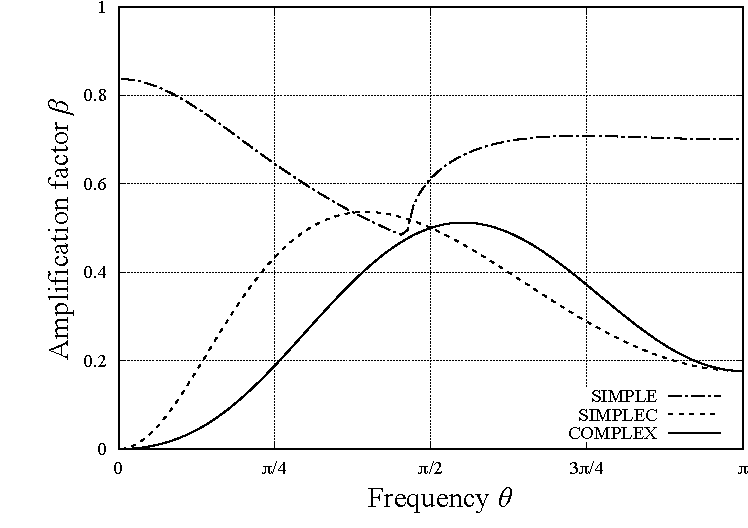
\includegraphics[width=0.45\textwidth]{fig/Re0001-b.pdf} \hspace{1cm}
    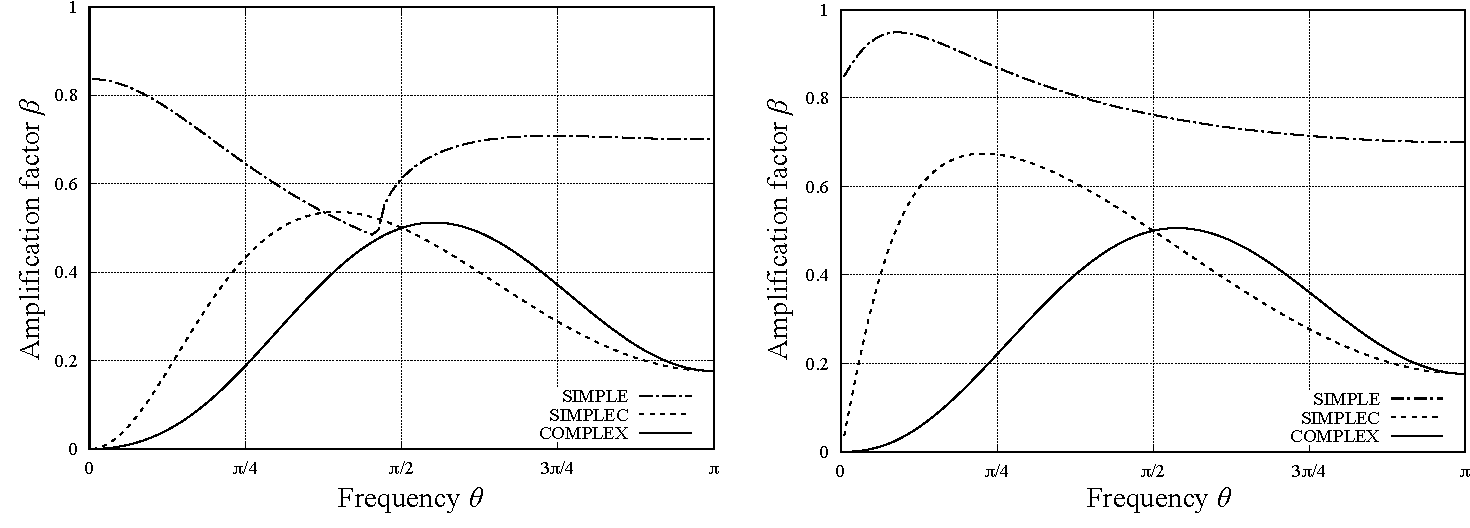
\includegraphics[width=\textwidth]{fig/Re_fourier.pdf}
    \caption{Amplification factor for $Re_h=0.001$ (left) and $Re_h=1000$ (right)}
    \label{fig:1a}
\end{figure}
    
Fig.~\ref{fig:1b} shows the sensitivity of the amplification factor to the momentum relaxation factor for all frequencies and for the three coupling methods. The results are obtained for a $Re_h=1$ and always considering the rule $\omega_P = 1 - \omega$ for SIMPLE. While the SIMPLE algorithm does not show any significant improvement for higher values of $\omega$ (even showing a range of instability for low frequencies at $\omega=0.95$ and $\omega_P=0.05$), the SIMPLEC algorithm shows a depletion in its performance for high momentum relaxation factors (tending to unity for $\theta=0$ as $\omega_u \rightarrow 1$). In this aspect, the COMPLEX algorithm shows a clear advantage over the other two methods by preserving almost unaltered the overall error damping, even for high momentum relaxation factors.     
    
\begin{figure}[t!!]
    \centering
    %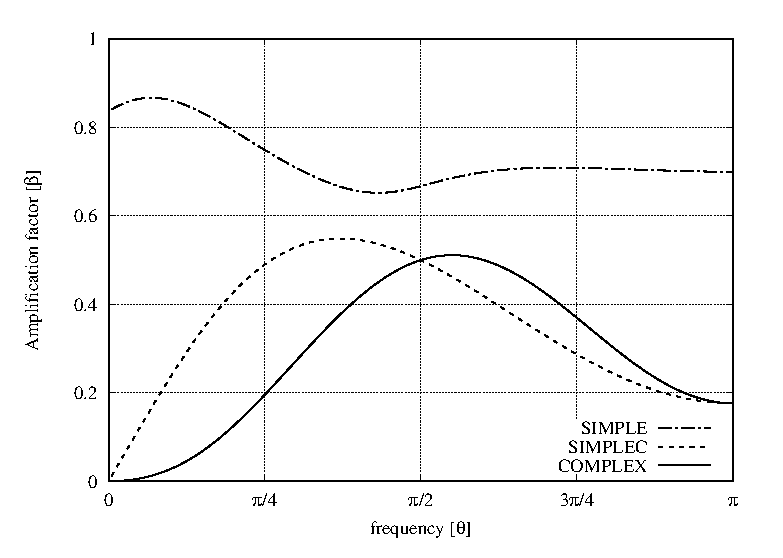
\includegraphics[width=0.45\textwidth]{fig/w07} \hspace{1cm}
    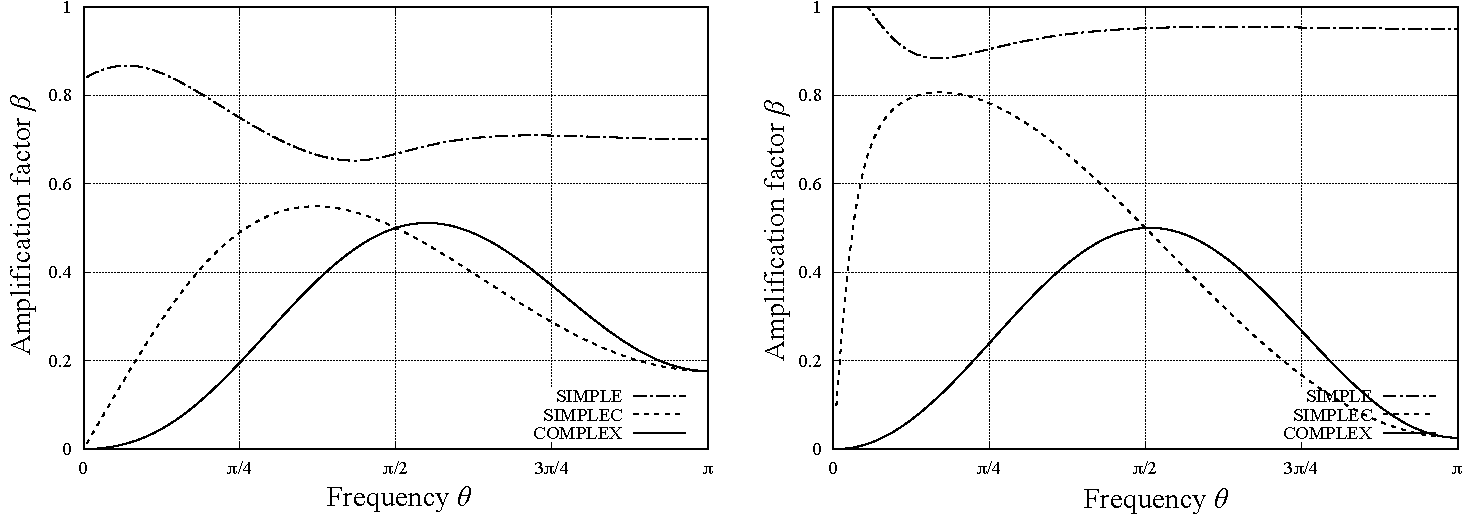
\includegraphics[width=\textwidth]{fig/w_fourier.pdf}
    \caption{Amplification factor for $\omega_u=0.7$ (left) and $\omega_u=0.95$ (right)}
    \label{fig:1b}
\end{figure}    

This theoretical advantage is very important since it indicates that the good performance of the method holds up even when the convergence rate to the steady state solution is accelerated by increasing the momentum relaxation factors. In the next section, this advantage will be put to the test in two benchmark tridimensional problems to verify the accuracy of these predictions on full CFD problems.

These analysis may be deepened by considering a continuous range as relaxation factors from $0$ to $1$ for the three methods, as shown in Fig. \ref{fig:1c}. These figures show a clear advantage of SIMPLEC over SIMPLE for almost every relaxation factor considered, and a clear advantage of COMPLEX over SIMPLEC for high values of the amplification factor. Here it may be noted that, for very low values of $\omega_u$ all methods tend to the same stability behavior.

\begin{figure}[b!]
    \centering
    \includegraphics[width=\textwidth]{fig/maps_fourier.pdf}
    \caption{Amplification factor for SIMPLE (a), SIMPLEC (b) and COMPLEX (c) for different relaxation factors and frequencies}
    \label{fig:1c}
\end{figure}    
    
A method to quantify the overall error damping for a general problem, where the initial solution is formed by an equally distributed amount of modes (i.e. assuming that there is no frequency that is clearly dominant over the others in the initial values of $u$ and $p$ fields), is to consider an frequency-average amplification factor. This is shown in Fig.~\ref{fig:1d}, where the mean value of $\beta$ over all frequencies is plotted for all the possible values of the momentum relaxation factor. Here it is also clear that, while all methods are stable under these conditions, the SIMPLEC and COMPLEX algorithms are clearly more efficient in terms of the error damping, and the COMPLEX algorithm outperforms SIMPLEC when the relaxation factor is increased. 

\begin{figure}[t!]
    \centering
    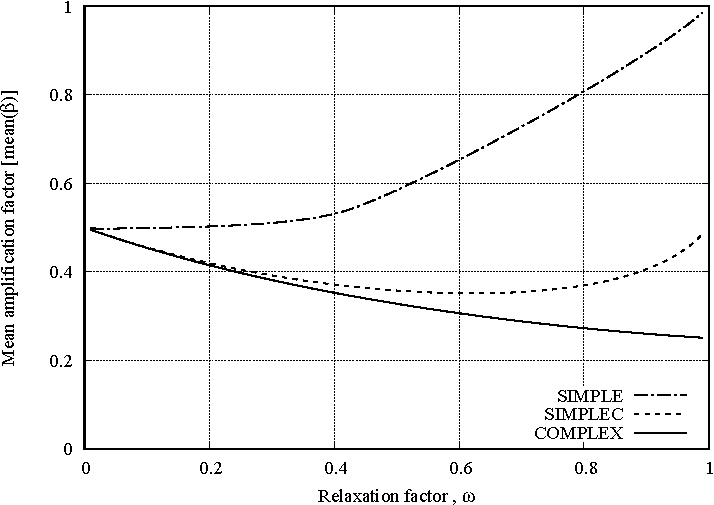
\includegraphics[width=0.5\textwidth]{fig/meanAmp.pdf}
    \caption{Mean amplification factor as a function of the momentum relaxation factor $\omega_u$}
    \label{fig:1d}
\end{figure}  

\section{Test cases}
\label{sec:cases}

In this section, the new pressure-velocity coupling strategy is analysed in the context of incompressible, laminar and stationary Newtonian flows. On this line, the numerical performance of the method is compared with  SIMPLE and SIMPLEC by evaluating the total number of iterations required to achieve a convergence criteria. First of all, the details of each problem are explained followed by the definition of the convergence criteria. Subsequently, the numerical configuration of the simulations are commented and after that, two different analysis over the COMPLEX method are performed. On the one hand, a serie of simulations are carried out to investigate a suitable value of the complex factor $\kappa$ and finally, a comparison of the current proposal with SIMPLE and SIMPLEC is presented for various conditions. 

\subsection{Test problems}\label{Section:problemDescription}
 The evaluation of the COMPLEX method is achieved by solving two typical tests for incompressible and stationary flows. The first of them is the cubic cavity test and the second one is the flow through the Backward Facing Step (BFS) channel.
\subsubsection{Cavity}
 A graphical scheme of this problem is depicted in Fig.~\ref{Fig:Cavity}.
\begin{figure}[t!!!]
\centering
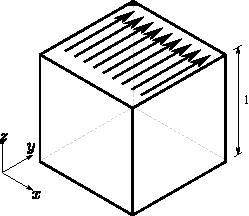
\includegraphics[width=5cm]{fig/Cases/Cavity.pdf}
\caption{The cubic cavity problem where a fixed tangential velocity is imposed on the upper face.}
\label{Fig:Cavity}
\end{figure} 
There, a tangential fixed velocity of 1 m/s is imposed on the upper face of the cubic domain of length 1 m. The case is solved using to different values of the kinematic viscosity, $\nu = 2.5\, e-3$ m$^2$/s and $\nu = 2.5$ m$^2$/s which defines the Reynolds number of 400 and $0.4$ respectively. For the purposes of this paper, the cavity is discretised with hexahedral cells using three different refinement levels: a coarse mesh with 25 divisions per side (15625 cells), a medium mesh with 50 divisions per side (125000 cells) and a fine mesh with 100 divisions per side (1000000 cells).

\subsubsection{Backward Facing Step}
The domain of this test and its dimension are shown in Fig.~\ref{Fig:Geometria3}.
\begin{figure}[t!!!]
\centering
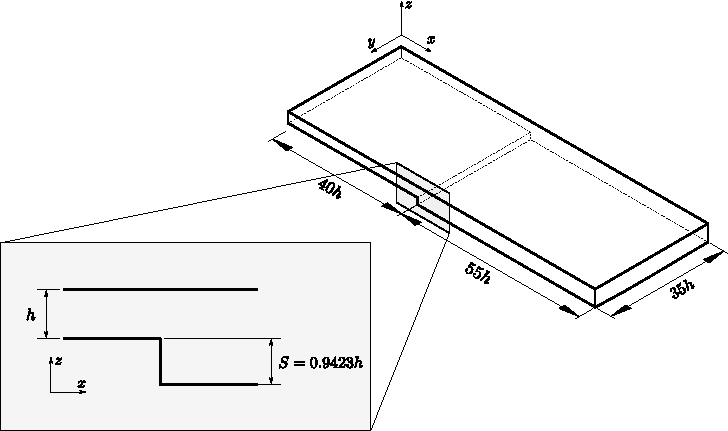
\includegraphics[width=12cm]{fig/Cases/Geometria3.pdf}
\caption{Description of the BFS domain where the dimensions are defined relative to the inlet height $h = 1$ m.}
\label{Fig:Geometria3}
\end{figure}
At the inlet, a constant and normal velocity of 1 m/s of magnitude is set up. Analogously to the cavity case, the problem is simulated with two different viscosity values, $\nu = 5.141\,e-3$ m$^2$/s and $\nu = 5.141$ m$^2$/s which refers to the Reynolds number of 389 and $0.389$ respectively. The BFS is discretized with hexahedral cells using three different mesh sizes as defined in Table~\ref{Table:BFSMeshes} with a variable cell size as plotted in Fig.~\ref{Fig:Factores} where the near wall regions and the step sector are relatively refined.
\begin{table}[b!]
\centering
\begin{tabular}{cccccccc}
\hline 
\multirow{2}{1cm}{Mesh Level} & \multicolumn{3}{c}{Pre-step divisions} & \multicolumn{3}{c}{Post-step divisions} & \multirow{2}{1cm}{Total Cells} \\ 
\cline{2-7} 
&  $x-$axis &  $y-$axis &  $z-$axis &  $x-$axis &  $y-$axis &  $z-$axis \\ 
\hline 
Coarse & 20 & 40 & 8 & 26 & 40 & 16 & 23040 \\ 
Medium & 40 & 80 & 15 & 52 & 80 & 30 & 172800 \\ 
Fine & 80 & 160 & 30 & 104 & 160 & 60 & 1382400 \\ 
\hline 
\end{tabular}
\caption{Scheme of divisions for the BFS case. The pre-step and post-step are the upstream and downstream regions of the step transversal section.}
\label{Table:BFSMeshes}
\end{table}

\begin{figure}[b!!!]
\centering
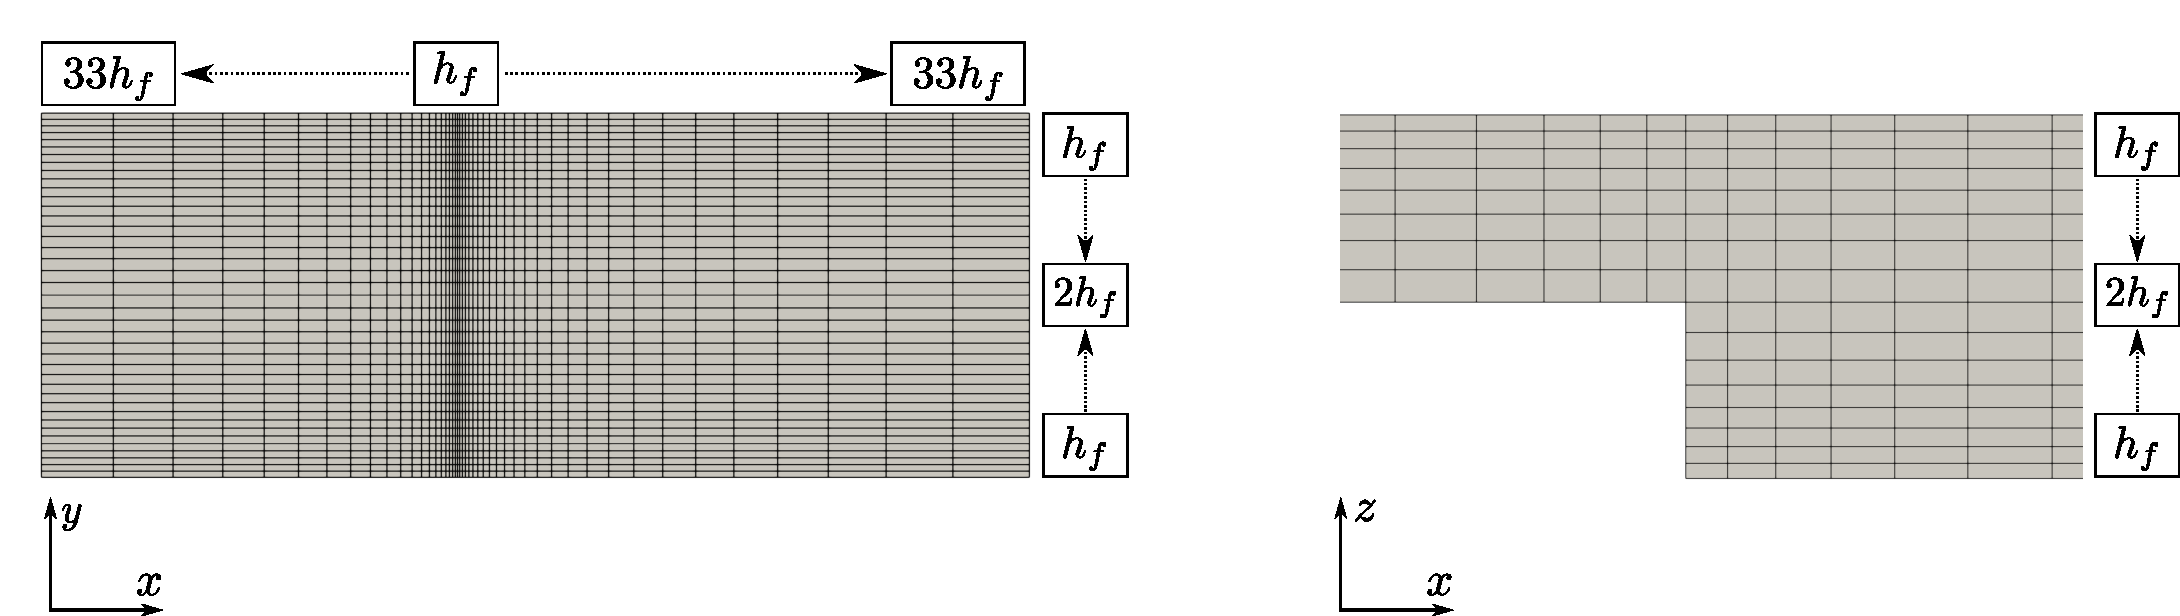
\includegraphics[width=16cm]{fig/Cases/Factores.pdf}
\caption{Variable cell refinement in the BFS.  On the left figure, the cell size grows from the step point up to the inlet and outlet boundaries and from the lateral walls up to the middle longitudinal section. On the right, the cell size in the post-step regions grows from the bottom and upper walls up to the middle height section of the channel.}
\label{Fig:Factores}
\end{figure}

\subsection{Error measurement}
To analyse the rate of convergence of the different algorithms, an error measure is defined. The error is assumed to be the residual of the discretized Navier-Stokes equations which are computed for each cell $P$ of the FV mesh $\Omega$. Then, the momentum residual writes,
\begin{equation}
\label{Eq:R1Discretized}
R_1(P)
=
\sum_{f}
\varphi_f\,
\boldsymbol{u}_p
+
\nu
\sum_f
\nabla \boldsymbol{u}_f
\cdot
\boldsymbol{S}_f
+
\sum_f
p_f
\,
\boldsymbol{S}_f
-
\boldsymbol{\Phi}_P \, V_P
\qquad \qquad
\forall P\,\in\,\Omega,
\end{equation}
and analogously, the mass residual may be computed as follows,
\begin{equation}
R_2(P)
=
\sum_f
\boldsymbol{u}_f
\cdot
\boldsymbol{S}_f
\qquad \qquad
\forall P\,\in\,\Omega,
\end{equation}
where the face velocity value $\boldsymbol{u}_f$ is replaced in terms of the momentum equation such as done in Eq.~(\ref{Eq:firstPressureEq}),
\begin{equation}
\label{Eq:R2Discretized}
R_2(P)
=
\sum_f 
\left(
\frac{1}{a_P}
\right)_f 
\nabla p_f
\cdot
\boldsymbol{S}_f 
-
\sum_f
\left(
\frac{\boldsymbol{H}_P}
{a_P}
\right)_f 
\cdot 
\boldsymbol{S}_f,
\qquad \qquad
\forall P\,\in\,\Omega.
\end{equation}
It is important to highlight that the computations of $R_1$ and $R_2$ are independent of the pressure-velocity coupling strategy employed. These equations are only function of the velocity and pressure values, and of the momentum equation coefficients which are equally assembled for the three pressure-velocity coupling methods studied in this paper. In addition to this, the residuals $R_1$ and $R_2$ are computed at the end of each time step of the simulation. 
On the basis of their definition, the residuals $R_1$ and $R_2$ are an appropriate indicator to qualify the convergence of the different numerical algorithms by isolating their specific influence. In particular of this paper, the Root Mean Square (RMS) value of them is computed, 
\begin{align}
\overline{R}_1
&=
\sqrt
{
\sum_{P\,\in\,\Omega}
R_1(P)^2
}
\\
\overline{R}_2
&=
\sqrt
{
\sum_{P\,\in\,\Omega}
R_2(P)^2
}.
\end{align}
Referring to the $\overline{R}_1$ and $\overline{R}_2$, the following convergence criteria is proposed in this work: a numerical simulation will be assumed as converged if both values, $\overline{R}_1$ and $\overline{R}_2$  are below a tolerance of $1e^{-9}$,
\begin{equation}
\label{Eq:convergenceCriteria}
\left\lbrace
\begin{array}{c}
\overline{R}_1 \leq 1e^{-9} \\
\overline{R}_2 \leq 1e^{-9}
\end{array}
\right..
\end{equation}

\subsection{Numerical setup}
The simulations of the different analysis are configured with the same numerical schemes. Namely, the convective terms are discretised with an upwind scheme and the pressure gradient operator is computed with a Gauss-based formula using linear interpolation to define the face values. Respecting the diffusive terms, they are discretized with a Gauss-based formula where the face gradient is assembled with a first-neighbour stencil. The linear system of equations are solved until a convergence of two order of magnitude is achieved for both, the momentum and mass balance systems. 

With reference to the relaxation factors, the momentum relaxation factor $\omega_u$ is a variable of the parametric study. On the other side, the pressure relaxation $\omega_p$ is equal to one in the COMPLEX and SIMPLEC simulations and in the SIMPLE ones it is defined as follows,
\begin{equation}
\label{Eq:relaxP}
\omega_p = 1 - \omega_u.
\end{equation}

  

\subsection{Study of the complex factor $\kappa$}
An important parameter of the current numerical method is the complex factor $\kappa$. In this study, the influence  of $\kappa$ on the convergence rate is analysed in combination with the relaxation factor for the momentum equation $\omega_{u}$ where the number of iterations required to reach the convergence criteria of Eq.~(\ref{Eq:convergenceCriteria}) is quantified.

The study solves a serie of simulations of the cavity and BFS problems using the medium refinement levels of the proposed meshes respectively. Furthermore, for each case, two different physical configuration are addressed according to the two Reynolds number proposed. Consequently, four different numerical problems are defined. Each one of this four simulations is solved varying the values of $\kappa$ and $\omega_{u}$. The complex factor is ranged from 0 to 1 by a step of $0.05$ (21 values) and the relaxation factor from 0.8 up to 1 by a step of $0.1$ (21 values) respectively. In combination, this parametric study is composed by 441 simulations for each one of the four numerical problems.

The results of the simulations are presented in the Tables~\ref{Table:Cavity_LowRe}, \ref{Table:BFS_LowRe}, \ref{Table:Cavity_HighRe} and \ref{Table:BFS_HighRe}, and in the Fig.~\ref{Fig:FactorLowRe}. One one hand, the tables present the required number of iterations to reach the convergence as function of $\omega_u$ and $\kappa$. Not all simulations are displayed due to space limitations, the range of $\omega_u$ is shortened from 0.92 to 1 and the $\kappa$ values are listed using a step of 0.1 instead of 0.05. On the other hand, the Fig.~\ref{Fig:FactorLowRe} present the results of the four cases using contour plots. There is one figure per case which plots the relative number of iterations ($RI$) required for each simulation compared with those required for the simulation with the same relaxation factor but with $\kappa = 0$. Formally, the relative iteration index $RI$ for a given pair of values $\omega_u$ and $\kappa$ is computed as follows,
\begin{equation}
\label{Eq:relativeIndex}
RI(\omega_u, \kappa)
=
\dfrac
{
NI(\omega_u, \kappa) - NI(\omega_u, 0)
}
{
NI(\omega_u, 0)
}
\times
100 \%,
\end{equation}
where $NI(\omega_u, \kappa)$ is the number of iterations required for convergence using the relaxation value $\omega_u$ and the complex factor $\kappa$ and $NI(\omega_u, 0)$ is the number of iterations required for the convergence using the relaxation value $\omega_u$ and a complex factor equal to $\kappa = 0$.

The Tables~\ref{Table:Cavity_LowRe},~\ref{Table:BFS_LowRe}, and the upper plots of Fig.~\ref{Fig:FactorLowRe} present the relative low Reynolds simulation results  and the Tables~\ref{Table:Cavity_HighRe},~\ref{Table:BFS_HighRe}, and the bottom plots of Fig.~\ref{Fig:FactorLowRe} present the relative high Reynolds ones. 
\begin{table}[b!!]
\centering
\begin{tabular}{c|ccccccccccc}
\hline 
$\omega_u$/$\kappa$ & 0 & 0.1 & 0.2 & 0.3 & 0.4 & 0.5 & 0.6 & 0.7 & 0.8 & 0.9 & 1 \\ 
\hline 
1 & div & div & div & div & div & div & div & div & div & div & div \\ 
0.99 & 1993 & 1702 & 1742 & 1754 & 1747 & 1742 & 1761 & div & div & div & div \\ 
0.98 & 991 & 842  & 845 & 856 & 866 & 870 & 870 & 868 & 865 & 863 & 864 \\ 
0.97 & 658 & 551  & 559 & 560 & 565 & 570 & 574 & 575 & 575 & 575 & 573 \\ 
0.96 & 491 &425  & 414 & 416 & 418 & 421 & 424 & 426 & 427 & 428 & 428 \\ 
0.95 & 391 & 348 & 327 & 330 & 332 & 333 & 335 & 337 & 338 & 339 & 339 \\ 
0.94 & 373 & 373 & 373 & 373 & 373 & 373 & 373 & 373 & 373 & 373 & 373 \\ 
0.93 & 438 & 438 & 438 & 438 & 438 & 438 & 438 & 438 & 438 & 438 & 438 \\ 
0.92 & 504 & 504 & 504 & 504 & 504 & 504 & 504 & 504 & 504 & 504 & 504 \\ 
\hline 
\end{tabular} 
\caption{Required number of iterations at convergence for the Cavity case with Re = $0.4$}
\label{Table:Cavity_LowRe}
\end{table}
\begin{table}[b!!]
\centering
\begin{tabular}{c|ccccccccccc}
\hline 
$\omega_u$/$\kappa$ & 0 & 0.1 & 0.2 & 0.3 & 0.4 & 0.5 & 0.6 & 0.7 & 0.8 & 0.9 & 1 \\ 
\hline 
1 & div & div & div & div & div & div & div & div & div & div & div \\ 
0.99 & 1974 & 1697 & 1753 & 1865 & 1941 & 1993 & div & div & div & div & div \\ 
0.98 & 981 & 816 & 844 & 854 & 874 & 904 & 929 & 949 & 966 & 980 & 992 \\ 
0.97 & 651 & 528 & 550 & 560 & 565 & 571 & 581 & 594 & 606 & 618 & 627 \\ 
0.96 & 486 & 392 & 403 & 413 & 418 & 421 & 424 & 428 & 435 & 442 & 449 \\ 
0.95 & 387 & 320 & 317 & 324 & 330 & 333 & 335 & 336 & 339 & 342 & 346 \\ 
0.94 & 320 & 272 & 259 & 266 & 271 & 274 & 276 & 277 & 278 & 280 & 282 \\ 
0.93 & 273 & 237 & 220 & 225 & 229 & 232 & 234 & 235 & 236 & 237 & 238 \\ 
0.92 & 240 & 233 & 233 & 233 & 233 & 233 & 233 & 233 & 233 & 233 & 233 \\ 
\hline 
\end{tabular}
\caption{Required number of iterations at convergence for the BFS case with Re = 0.389}
\label{Table:BFS_LowRe}
\end{table}
\begin{table}[t!!]
\centering
\begin{tabular}{c|ccccccccccc}
\hline 
$\omega_u$/$\kappa$ & 0 & 0.1 & 0.2 & 0.3 & 0.4 & 0.5 & 0.6 & 0.7 & 0.8 & 0.9 & 1 \\ 
\hline 
1 & div & div & div & div & div & div & div & div & div & div & div \\ 
0.99 & 1611 & 1321 & 1286 & 1333 & 1357 & div & div & div & div & div & div \\ 
0.98 & 802 & 693 & 652 & 635 & 648 & 662 & 671 & 678 & 682 & div & div \\ 
0.97 & 532 & 471 & 448 & 431 & 423 & 427 & 435 & 441 & 446 & 449 & 452 \\ 
0.96 & 398 & 357 & 342 & 330 & 321 & 317 & 319 & 323 & 327 & 331 & 333 \\ 
0.95 & 318 & 288 & 277 & 269 & 262 & 257 & 255 & 256 & 258 & 261 & 263 \\ 
0.94 & 266 & 243 & 235 & 229 & 225 & 221 & 218 & 216 & 215 & 216 & 217 \\ 
0.93 & 239 & 225 & 218 & 214 & 211 & 211 & 211 & 210 & 210 & 210 & 209 \\ 
0.92 & 243 & 243 & 242 & 242 & 242 & 241 & 241 & 241 & 241 & 241 & 240 \\ 
\hline 
\end{tabular}
\caption{Required number of iterations at convergence for the Cavity case with Re = 400}
\label{Table:Cavity_HighRe}
\end{table}
\begin{table}[t!!]
\centering
\begin{tabular}{c|ccccccccccc}
\hline 
$\omega_u$/$\kappa$ & 0 & 0.1 & 0.2 & 0.3 & 0.4 & 0.5 & 0.6 & 0.7 & 0.8 & 0.9 & 1 \\ 
\hline 
1 & div & div & div & div & div & div & div & div & div & div & div \\ 
0.99 & div & div & div & div & div & div & div & div & div & div & div \\ 
0.98 & 818 & 624 & 632 & 637 & div & div & div & div & div & div & div \\ 
0.97 & 540 & 427 & 422 & 428 & 435 & div & div & div & div & div & div \\ 
0.96 & 403 & 329 & 323 & 327 & 329 & 478 & 3086 & div & div & div & div \\ 
0.95 & 322 & 272 & 264 & 266 & 268 & 351 & 712 & 4714 & div & div & div \\ 
0.94 & 269 & 236 & 227 & 226 & 250 & 320 & 483 & 1151 & div & div & div \\ 
0.93 & 240 & 225 & 218 & 221 & 246 & 299 & 397 & 608 & 1427 & div & div \\ 
0.92 & 242 & 235 & 230 & 232 & 256 & 292 & 351 & 457 & 696 & 1087 & 8863 \\ 
\hline 
\end{tabular}
\caption{Required number of iterations at convergence for the BFS case with Re = 389}
\label{Table:BFS_HighRe}
\end{table}
\begin{figure}[t!!!!!!!]
\centering
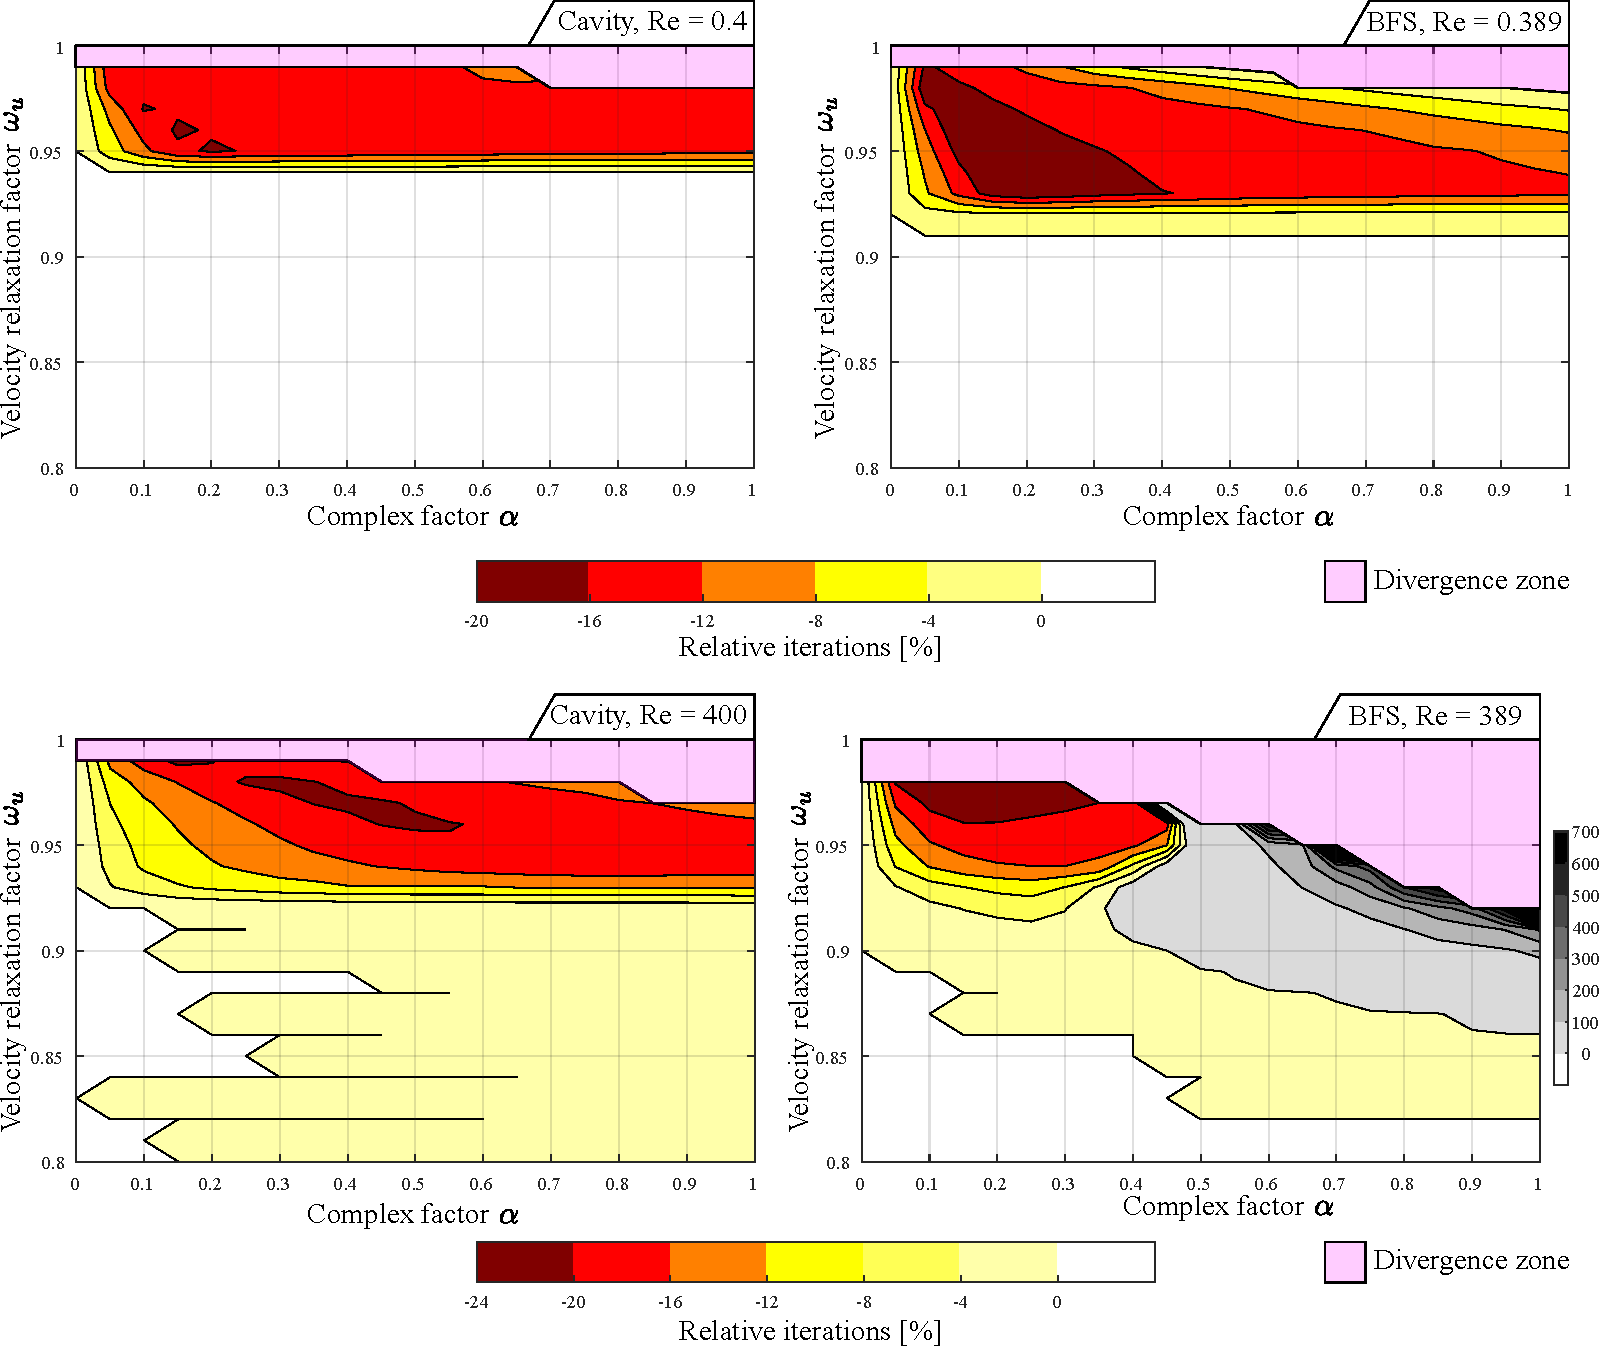
\includegraphics[width=17cm]{fig/Results/FactorLowRe.pdf}
\caption{Isolines of relative iterations as function of the momentum relaxation factor and the complex factor for the Cavity and BFS cases and the values of the Reynolds number employed respectively.}
\label{Fig:FactorLowRe}
\end{figure}
In general, it is concluded that the addition of the complex term does not influence the convergence when using relative low relaxation factors. On the contrary, with relative high values of $\omega_u$, the addition of the complex term reduces the number of iterations required for convergence. This reduction has a maximum value of approximately 20 $\%$ in the total number of iterations. The better results are obtained with values of the complex factor that are below $k = 0.5$. The simulations with high values of the complex factor $(k \geq 0.5)$ may be unstable. In particular, the BFS problem at Re = 389 indicates an extended divergence zone for the highest values of $\omega_u$ which is followed by a slow convergence zone (grey-coloured zone in the figure) for lower values of $\omega_u$. Unlike this last behavour, with lower values of $\kappa$, the simulations are stable and indicate the maximum convergence speed. 

In view of this investigation, it is concluded that a complex factor equal to $\kappa = 0.2$ is adequate to speed up the convergence without losing stability. This last inference is determined based on two different numerical problems (Cavity and BFS) in the range of Reynolds number between $0.4$ and $400$. 

 
\subsection{Comparison of COMPLEX with SIMPLE and SIMPLEC}
In the next paragraphs, a comparison of the COMPLEX strategy against the SIMPLE and SIMPLEC methods is performed. Here, the COMPLEX	 simulations are solved using a complex factor of $\kappa = 0.2$. 
Similar as solved in the previous section, the number of iterations required to reach the convergence criteria is measured. Each of the four numerical cases defined in previous section is solved using the coarse, medium and fine mesh levels. As well as the Reynolds number and the mesh refinement, the effect of momentum relaxation factor on the convergence is included into the exploration. Therefore, the simulations are solved varying $\omega_u$ from 0.8 to 1 using a step of 0.1.
\begin{figure}[t!]
\centering
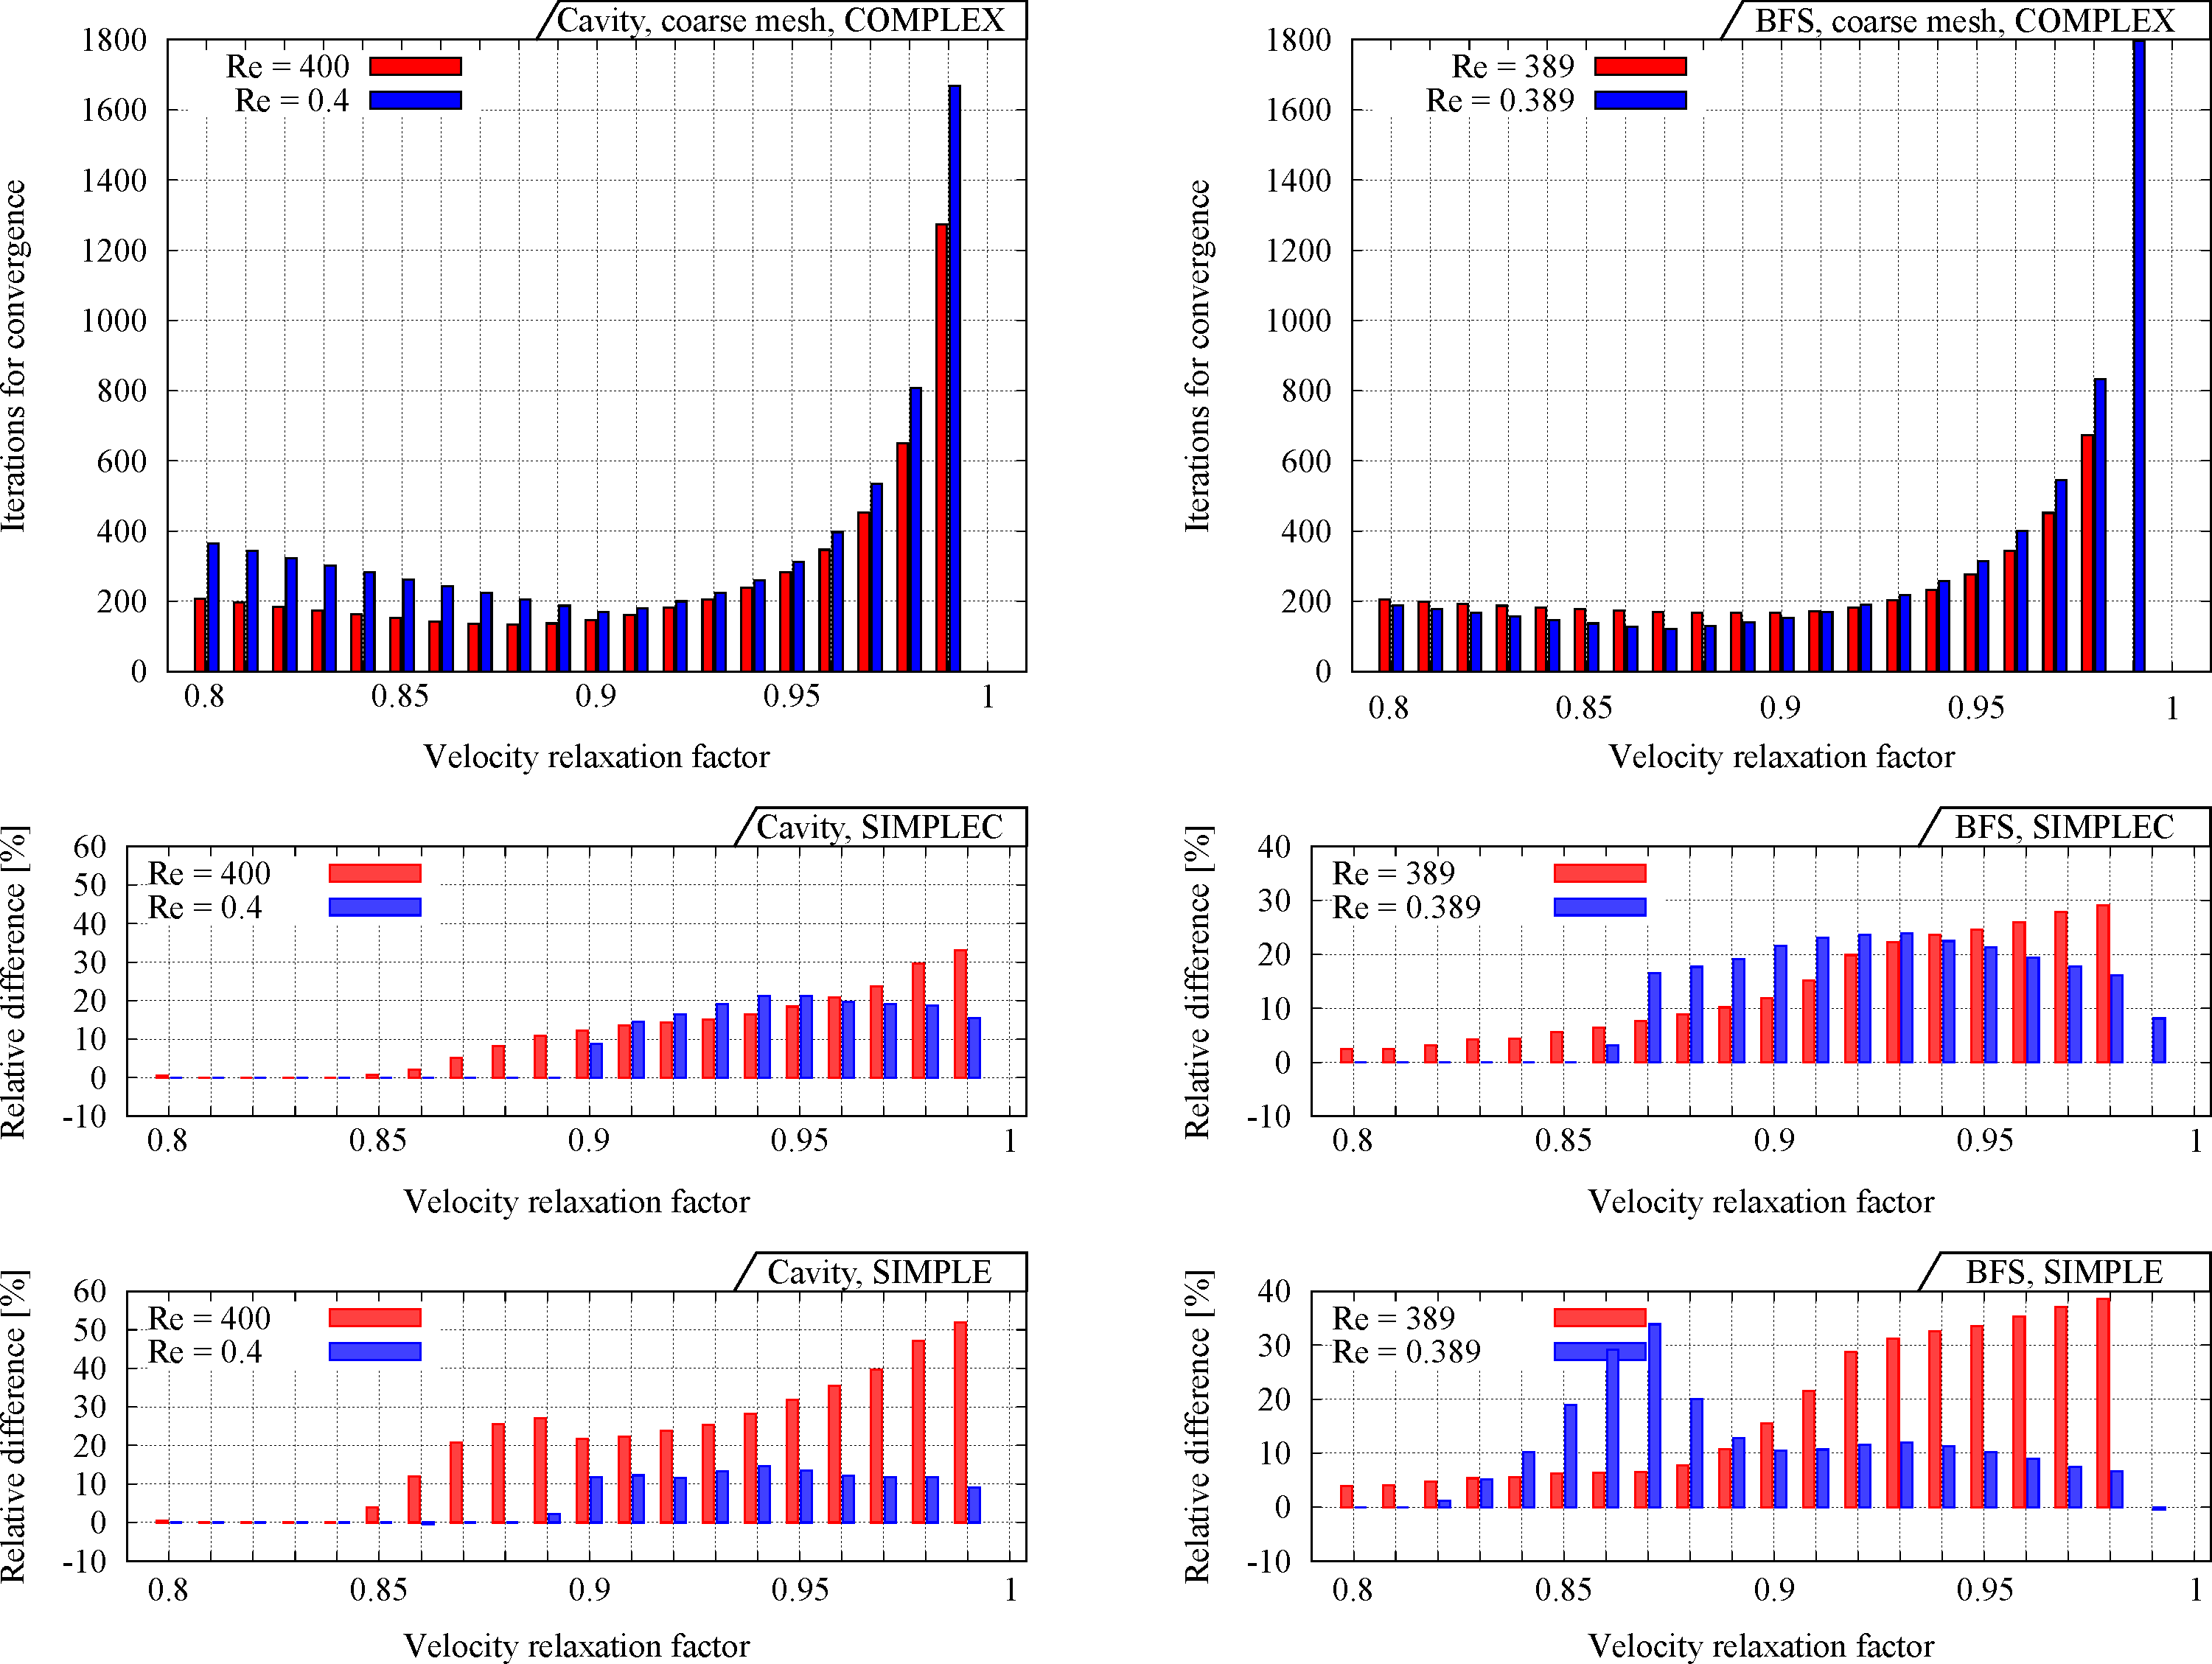
\includegraphics[width=17cm]{fig/Results/complexCoarse.pdf}
\caption{Comparison of the number of iterations required for convergence between COMLEX, SIMPLEC and SIMPLE algorithms using the coarse mesh refinement level. On the left are the results of the Cavity case and on the right, those respective to the BFS.}
\label{Fig:complexCoarse}
\end{figure}

\begin{figure}[t!]
\centering
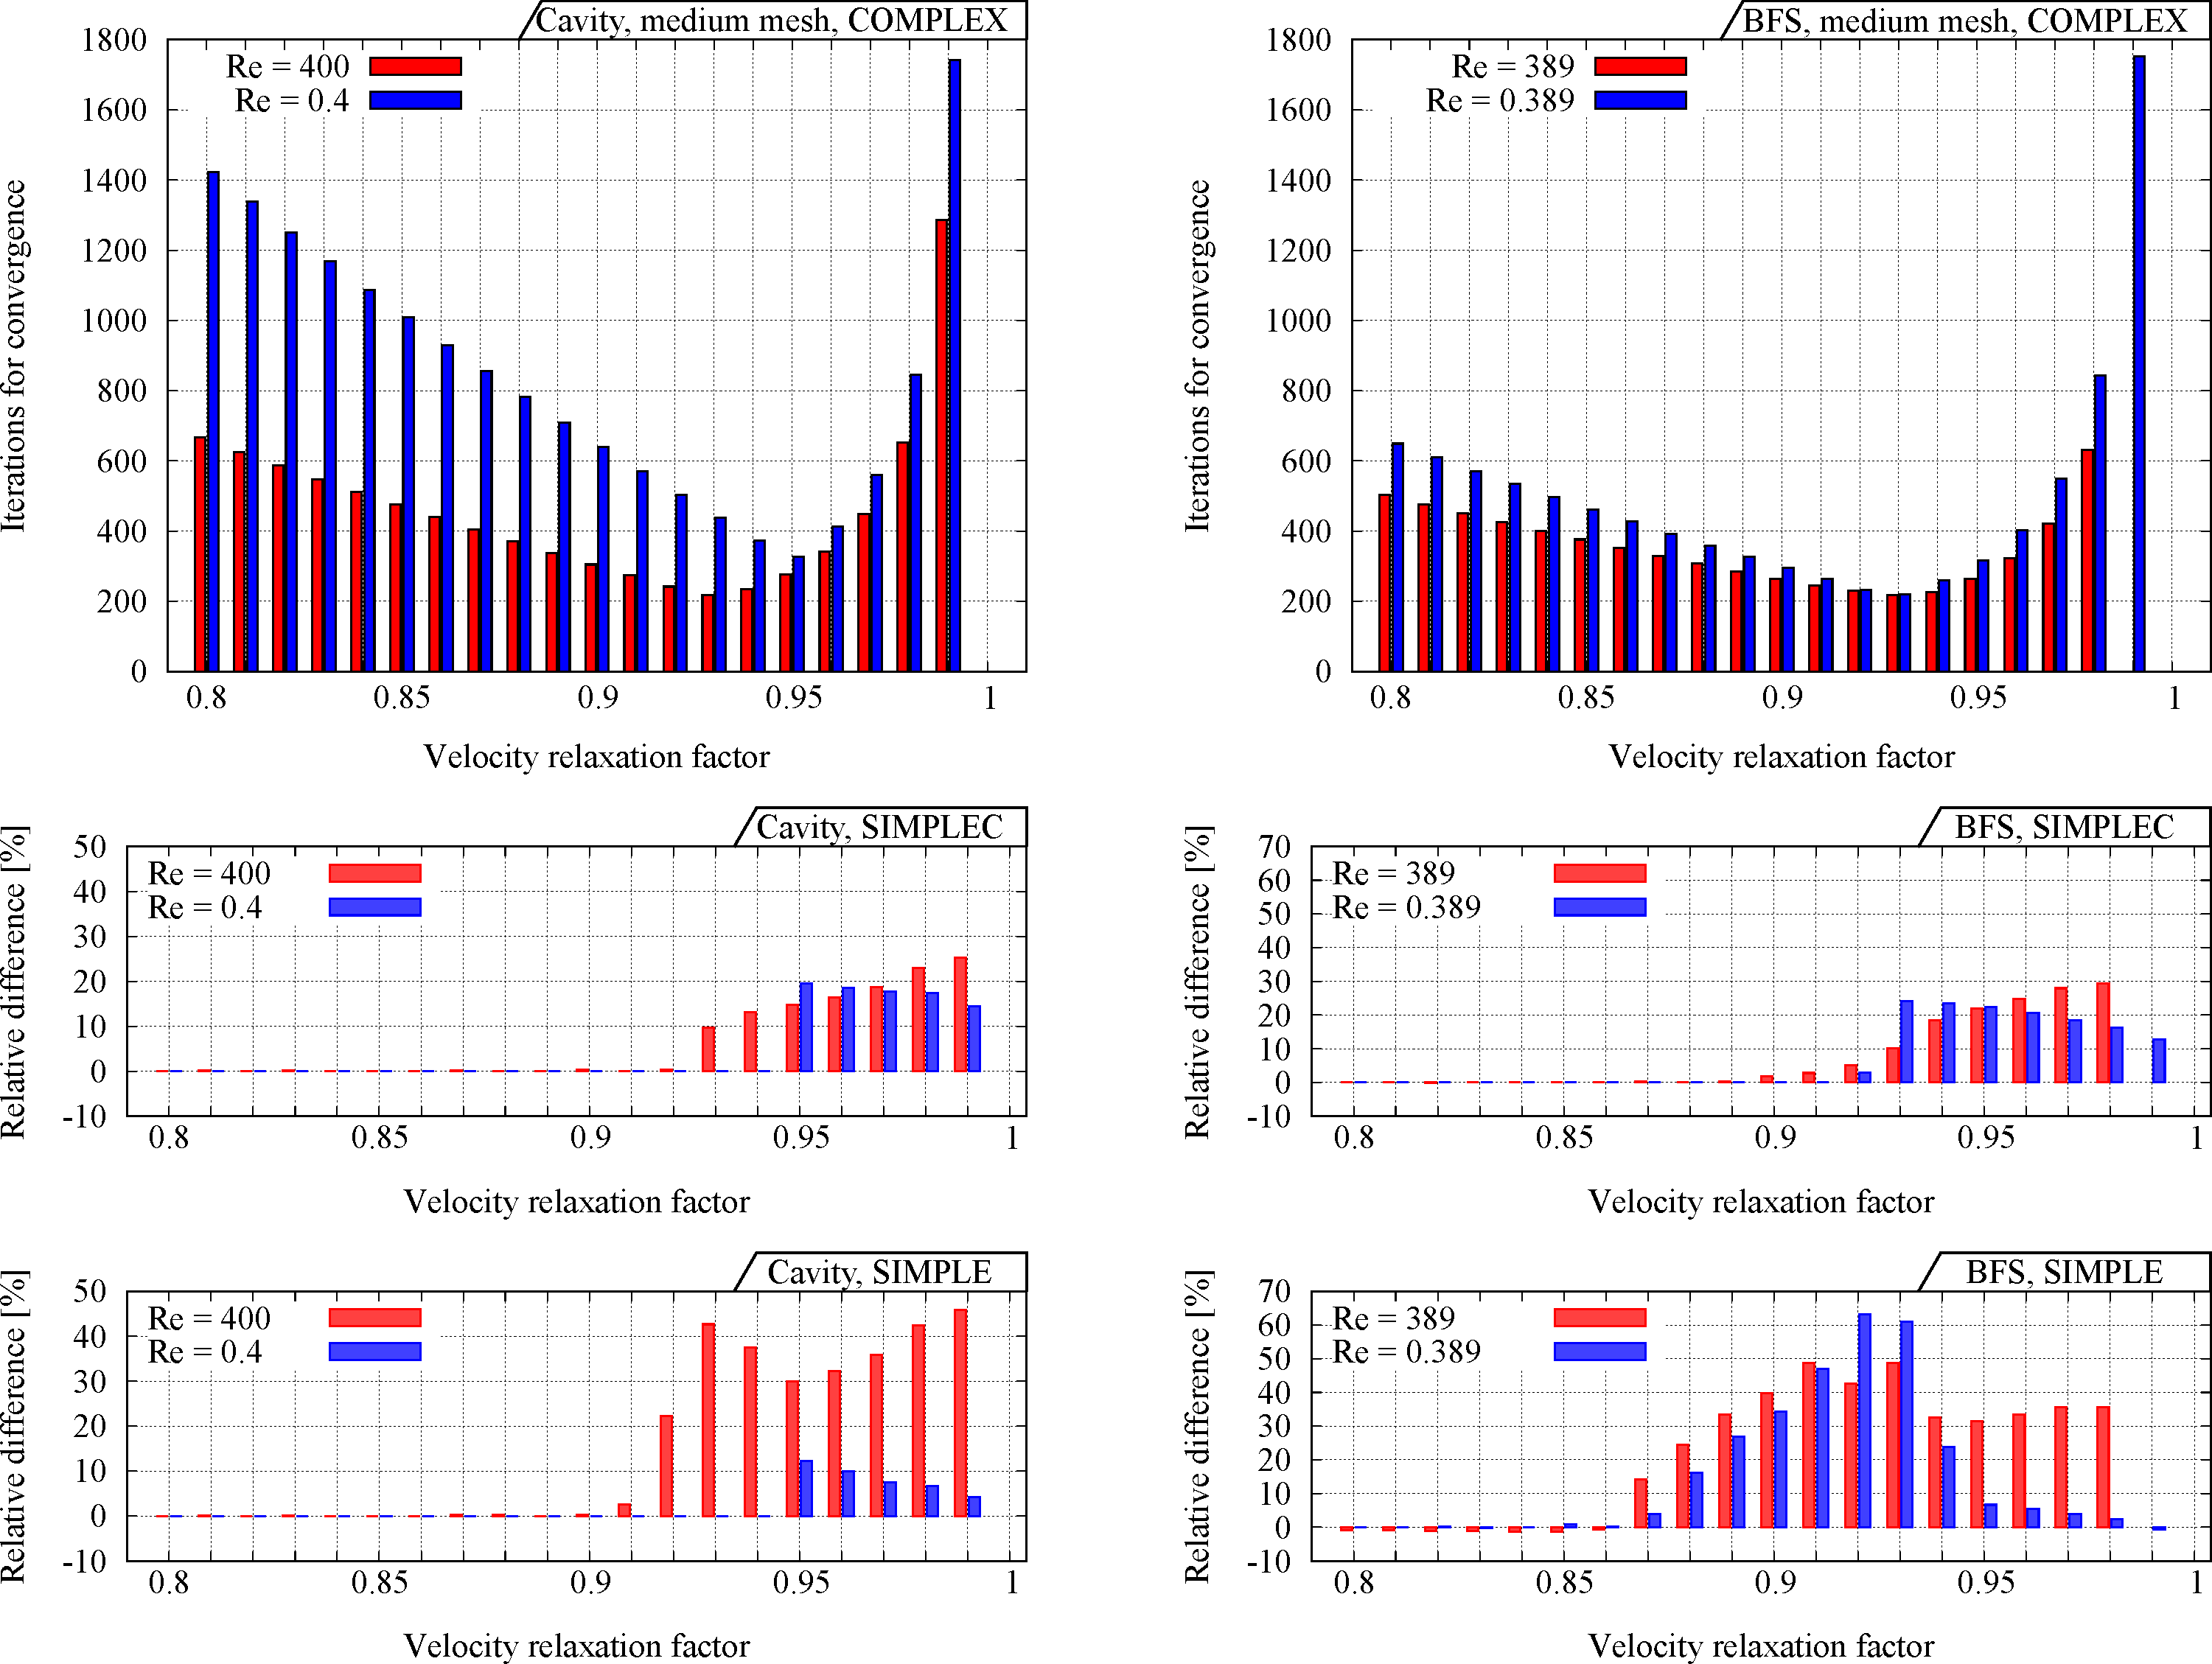
\includegraphics[width=17cm]{fig/Results/complexMedium.pdf}
\caption{Comparison of the number of iterations required for convergence between COMLEX, SIMPLEC and SIMPLE algorithms using the medium mesh refinement level. On the left are the results of the Cavity case and on the right, those respective to the BFS.}
\label{Fig:complexMedium}
\end{figure}

\begin{figure}[t!]
\centering
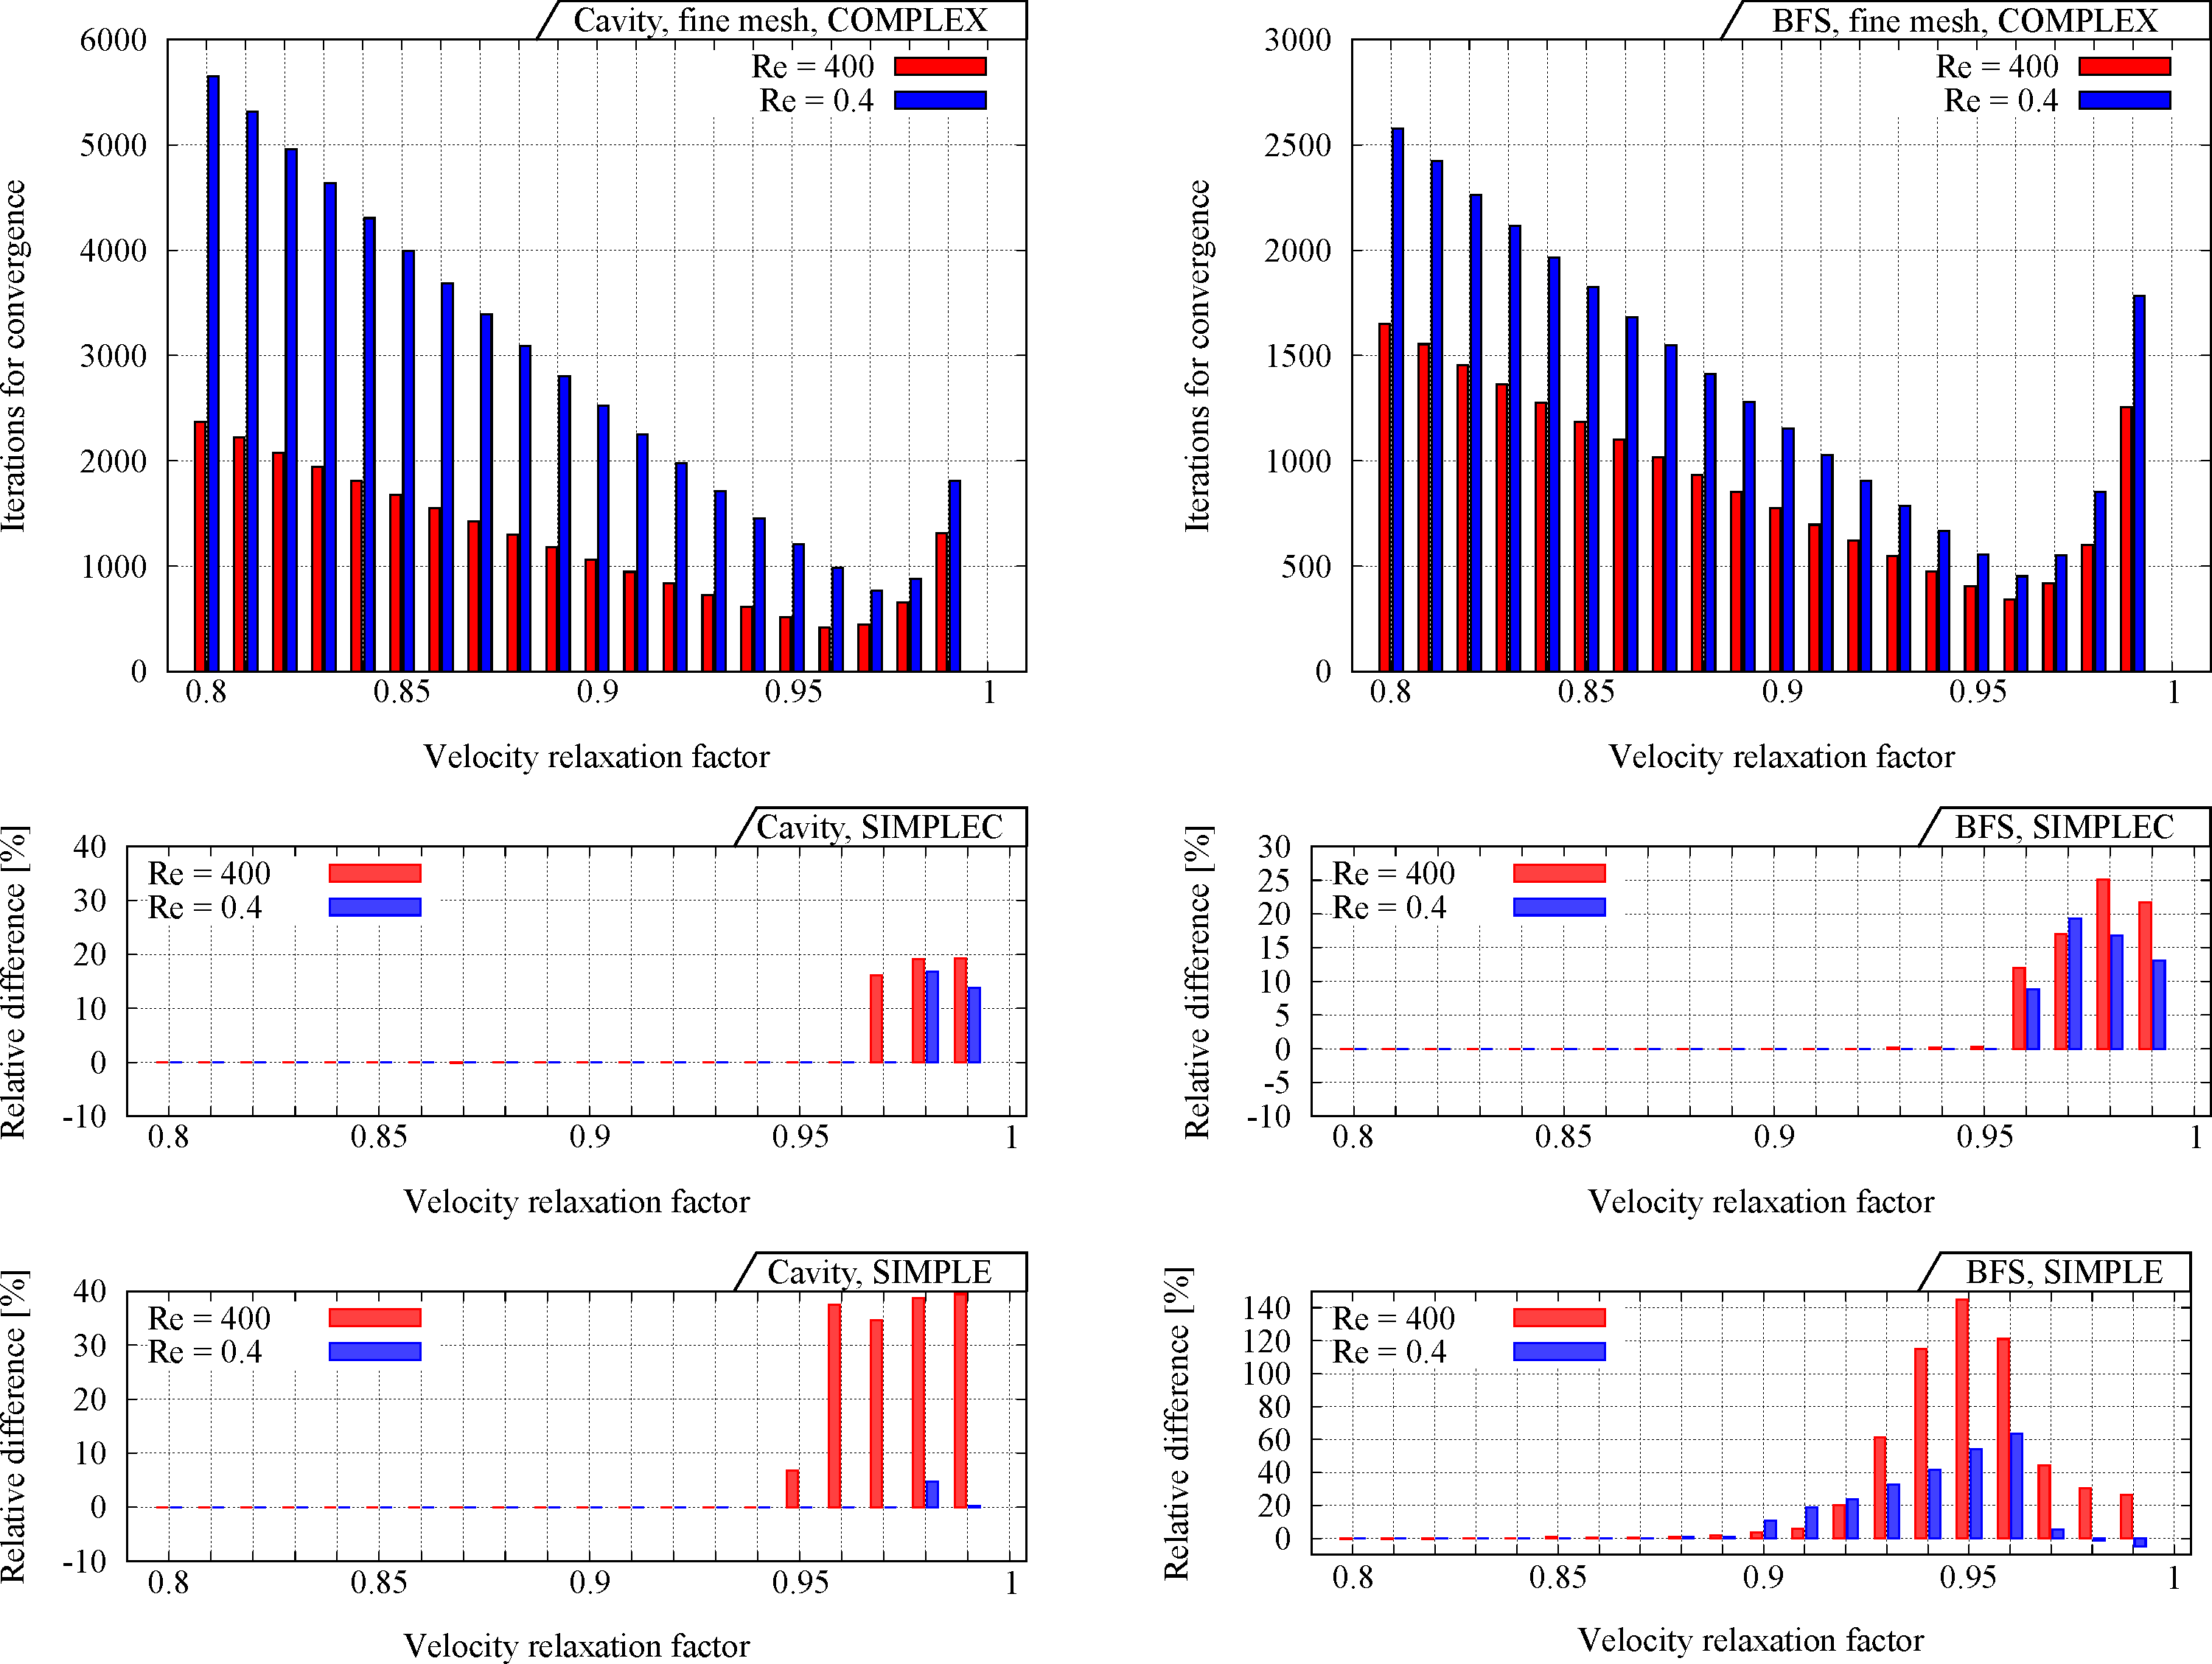
\includegraphics[width=17cm]{fig/Results/complexFine.pdf}
\caption{Comparison of the number of iterations required for convergence between COMLEX, SIMPLEC and SIMPLE algorithms using the fine mesh refinement level. On the left are the results of the Cavity case and on the right, those respective to the BFS.}
\label{Fig:complexFine}
\end{figure}

The results are presented in the Figs.~\ref{Fig:complexCoarse},~\ref{Fig:complexMedium} and \ref{Fig:complexFine} which are respective to the three refinement mesh levels. Each figure includes six bar plots arranged in three rows and two columns. On the right and left columns, the results of the Cavity and BFS simulations are presented respectively. In the first row, the absolute number of iterations at convergence for the COMPLEX method simulations are indicated. Relative to these simulations, the second and third row display the relative number of iterations in percentage for the SIMPLEC and SIMPLE methods respectively,
\begin{equation}
RI(\omega_u)
=
\dfrac
{NI_S(\omega_u) - NI_C(\omega_u)}
{NI_C(\omega_u)}
\times
100\%,
\end{equation}
where $NI_S(\omega_u)$ is the absolute number of iterations required at convergence for the SIMPLEC or SIMPLE method as appropriate when using a relaxation factor of momentum equal to $\omega_u$ and $NI(\omega_u)_C$. 
 In all plots, the blue bars are respective to the relative low Reynolds simulations while the red ones are respective to the relative high Reynolds ones.   

In general, the difference between COMPLEX and the other studied methods is relevant for high values of the momentum relaxation factor $\omega_u$. Examining the absolute number of iterations of COMPLEX, the  value of $\omega_u$ in which the complex method has the best convergence is coincident with the start point from which the differences between the methods become significant. This last observation may be interpreted as COMPLEX has a lower minimum of the required iterations in order to converge and that the decay of the convergence caused by an excessive value of $\omega_u$ is better handled by the COMPLEX method. An hypothesis for the previous reaction of the methods may be explained by considering that a higher relaxation factor of the momentum equation leads to a higher divergence of the velocity field, since this constraint is naturally not imposed in the momentum balance. With this in mind, the COMPLEX strategy includes a numerical correction for this deviation which helps to an enhanced prediction of the pressure in these conditions.

The results are sensitive to the mesh refinement level. Analysing the absolute number of iterations of the COMPLEX method, it is observed that the reduction of the number of iterations when increasing the momentum relaxation factor raises up with mesh refinement. This also deviates the minimum iterations point to the right direction in concordance with a higher value of $\omega_u$. 

The mesh refinement level affects the relative differences between the methods. The range of $\omega_u$ in which COMPLEX converges better is wider in the coarse mesh than in the fine mesh. Namely, this range start from $\omega_u = 0.85$ in the coarse mesh and from $\omega_u = 0.95$ in the fine one.

In regard to the Reynolds number influence on COMPLEX it may be assert that for the relative high Reynolds number, a less iterations are required to reach the convergence criteria. This property of COMPLEX is also observed when comparing it with SIMPLE and SIMPLEC. Here, the iteration reduction required for convergence is higher for the relative high Reynold problems. A similar effect is also noted in the range in which COMPLEX is more convergent. As pointed out before, the range of advantage of COMPLEX regarding the $\omega_u$ value starts at the point where the iteration number is approaching a minimum. This trend is also observed in the high Reynolds simulations since the wider range of advantage of COMPLEX compared with the low Reynolds problems may be justified since the minimum iterations number occurs with a lower value of $\omega_u$.

%To conclude this analysis, it is remarked that in almost all cases (Cavity or BFS, mesh refinement level $\omega_u$ value, and Reynolds number) the COMPLEX method is superior in terms of convergence than both, the SIMPLE and SIMPLEC method.

To finalize this section, a further analysis of the COMPLEX method is performed by studying its computational efficiency. The  COMPLEX algorithm was implemented using the OpenFOAM(R)  libraries for the FVM \cite{ofpg}. In this sense, the current implementation of COMPLEX is compared with the OpenFOAM(R) reference of SIMPLEC. In this comparison, it is measured that COMPLEX  has a relative increment of the computational time per iteration of approximately 5$\%$ when solving the problems of this section. In them, the maximum computational performance is obtained when using high values of the momentum relaxation factor. Comparing the maximum performance of each one of the algorithms, the COMPLEX method saves between 10$\%$ and 20$\%$ of iterations which leads to a better computational efficiency.


\section{Conclusions}
\label{sec:conclusions}
This paper presents a new segregated algorithm, called COMPLEX, to solve incompressible flow problems using the FVM. It is based on SIMPLEC where the neighbour velocity approximation is enhanced using a first-order Taylor series expansion. The current procedure requires computing a velocity derivative which is simplified to a scalar matrix and defined solving a mass balance. The contribution of the first-order term of the Taylor expansion is included in the pressure equation. This terms is relaxed by the so-called complex factor $\kappa$.  

The stability of the COMPLEX method is compared against the SIMPLE and SIMPLEC ones via a Fourier decomposition of the error in one-dimensional cases. This study prompts that, for low momentum relaxation factors, both SIMPLEC and COMPLEX behave similarly but, for high momentum relaxation factors, the COMPLEX method has a better performance in terms of error damping. This indicates that, under the hypothesis of the Fourier analysis, the current method would have a higher convergence rate.

Additionally, two three-dimensional problems at different flow regimes were solved: a cubic cavity and a BFS test. Firstly, the optimal value of the Complex relaxation factor $\kappa$ was investigated. To do this, an exhaustive study of more than 1500 simulations was performed where the total number of iterations was measured for different values of the momentum relaxation factor, the Complex relaxation factor $\kappa$ and the Reynolds number. Based on the results, a Complex relaxation factor of $\kappa = 0.2$ was chosen as the most suitable for the problems under study. Secondly, the performance of the COMPLEX method was compared with SIMPLE and SIMPLEC. Here, each problem was solved using three different mesh refinements for the low and high values of the Reynolds number. The results proved that the COMPLEX method has a better convergence rate for high values of the momentum relaxation factor, which verifies the results of the Fourier analysis. This advantage prevails for a wider range of relaxation factors in the coarsest mesh. For the cases under study, the COMPLEX method shows a better convergence for the problems with the high Reynolds number. Here, the advantages over the standard SIMPLE algorithm are remarkable.

Based on the results of the present work, the current strategy is a promising technique to speed up the convergence of segregated algorithms. Its computational implementation is simple and it does not introduce a significant computational cost compared with the SIMPLEC method. The convergence rate of COMPLEX is better than SIMPLEC and SIMPLE when the prediction of the velocity is far from verifying the divergence free condition, as it is the case of high relaxation factors or high Reynolds numbers. 
A challenge for future works consists on improving the prediction of the velocity derivative in the Taylor series expansion. One alternative may be to follow the strategy of this work by proposing an improved  approximation of Eq.~(\ref{Eq:scalarMatrix}) to allow an anisotropic deformation of the velocity correction. On the other hand, other numerical approaches may be explored to compute the velocity gradient, for example, an expression based on a second derivative of the pressure. 

\bibliographystyle{unsrtnat}
\bibliography{main}

\end{document}
